\documentclass[1p]{elsarticle_modified}
%\bibliographystyle{elsarticle-num}

%\usepackage[colorlinks]{hyperref}
%\usepackage{abbrmath_seonhwa} %\Abb, \Ascr, \Acal ,\Abf, \Afrak
\usepackage{amsfonts}
\usepackage{amssymb}
\usepackage{amsmath}
\usepackage{amsthm}
\usepackage{scalefnt}
\usepackage{amsbsy}
\usepackage{kotex}
\usepackage{caption}
\usepackage{subfig}
\usepackage{color}
\usepackage{graphicx}
\usepackage{xcolor} %% white, black, red, green, blue, cyan, magenta, yellow
\usepackage{float}
\usepackage{setspace}
\usepackage{hyperref}

\usepackage{tikz}
\usetikzlibrary{arrows}

\usepackage{multirow}
\usepackage{array} % fixed length table
\usepackage{hhline}

%%%%%%%%%%%%%%%%%%%%%
\makeatletter
\renewcommand*\env@matrix[1][\arraystretch]{%
	\edef\arraystretch{#1}%
	\hskip -\arraycolsep
	\let\@ifnextchar\new@ifnextchar
	\array{*\c@MaxMatrixCols c}}
\makeatother %https://tex.stackexchange.com/questions/14071/how-can-i-increase-the-line-spacing-in-a-matrix
%%%%%%%%%%%%%%%

\usepackage[normalem]{ulem}

\newcommand{\msout}[1]{\ifmmode\text{\sout{\ensuremath{#1}}}\else\sout{#1}\fi}
%SOURCE: \msout is \stkout macro in https://tex.stackexchange.com/questions/20609/strikeout-in-math-mode

\newcommand{\cancel}[1]{
	\ifmmode
	{\color{red}\msout{#1}}
	\else
	{\color{red}\sout{#1}}
	\fi
}

\newcommand{\add}[1]{
	{\color{blue}\uwave{#1}}
}

\newcommand{\replace}[2]{
	\ifmmode
	{\color{red}\msout{#1}}{\color{blue}\uwave{#2}}
	\else
	{\color{red}\sout{#1}}{\color{blue}\uwave{#2}}
	\fi
}

\newcommand{\Sol}{\mathcal{S}} %segment
\newcommand{\D}{D} %diagram
\newcommand{\A}{\mathcal{A}} %arc


%%%%%%%%%%%%%%%%%%%%%%%%%%%%%5 test

\def\sl{\operatorname{\textup{SL}}(2,\Cbb)}
\def\psl{\operatorname{\textup{PSL}}(2,\Cbb)}
\def\quan{\mkern 1mu \triangleright \mkern 1mu}

\theoremstyle{definition}
\newtheorem{thm}{Theorem}[section]
\newtheorem{prop}[thm]{Proposition}
\newtheorem{lem}[thm]{Lemma}
\newtheorem{ques}[thm]{Question}
\newtheorem{cor}[thm]{Corollary}
\newtheorem{defn}[thm]{Definition}
\newtheorem{exam}[thm]{Example}
\newtheorem{rmk}[thm]{Remark}
\newtheorem{alg}[thm]{Algorithm}

\newcommand{\I}{\sqrt{-1}}
\begin{document}

%\begin{frontmatter}
%
%\title{Boundary parabolic representations of knots up to 8 crossings}
%
%%% Group authors per affiliation:
%\author{Yunhi Cho} 
%\address{Department of Mathematics, University of Seoul, Seoul, Korea}
%\ead{yhcho@uos.ac.kr}
%
%
%\author{Seonhwa Kim} %\fnref{s_kim}}
%\address{Center for Geometry and Physics, Institute for Basic Science, Pohang, 37673, Korea}
%\ead{ryeona17@ibs.re.kr}
%
%\author{Hyuk Kim}
%\address{Department of Mathematical Sciences, Seoul National University, Seoul 08826, Korea}
%\ead{hyukkim@snu.ac.kr}
%
%\author{Seokbeom Yoon}
%\address{Department of Mathematical Sciences, Seoul National University, Seoul, 08826,  Korea}
%\ead{sbyoon15@snu.ac.kr}
%
%\begin{abstract}
%We find all boundary parabolic representation of knots up to 8 crossings.
%
%\end{abstract}
%\begin{keyword}
%    \MSC[2010] 57M25 
%\end{keyword}
%
%\end{frontmatter}

%\linenumbers
%\tableofcontents
%
\newcommand\colored[1]{\textcolor{white}{\rule[-0.35ex]{0.8em}{1.4ex}}\kern-0.8em\color{red} #1}%
%\newcommand\colored[1]{\textcolor{white}{ #1}\kern-2.17ex	\textcolor{white}{ #1}\kern-1.81ex	\textcolor{white}{ #1}\kern-2.15ex\color{red}#1	}

{\Large $\underline{12a_{0918}~(K12a_{0918})}$}

\setlength{\tabcolsep}{10pt}
\renewcommand{\arraystretch}{1.6}
\vspace{1cm}\begin{tabular}{m{100pt}>{\centering\arraybackslash}m{274pt}}
\multirow{5}{120pt}{
	\centering
	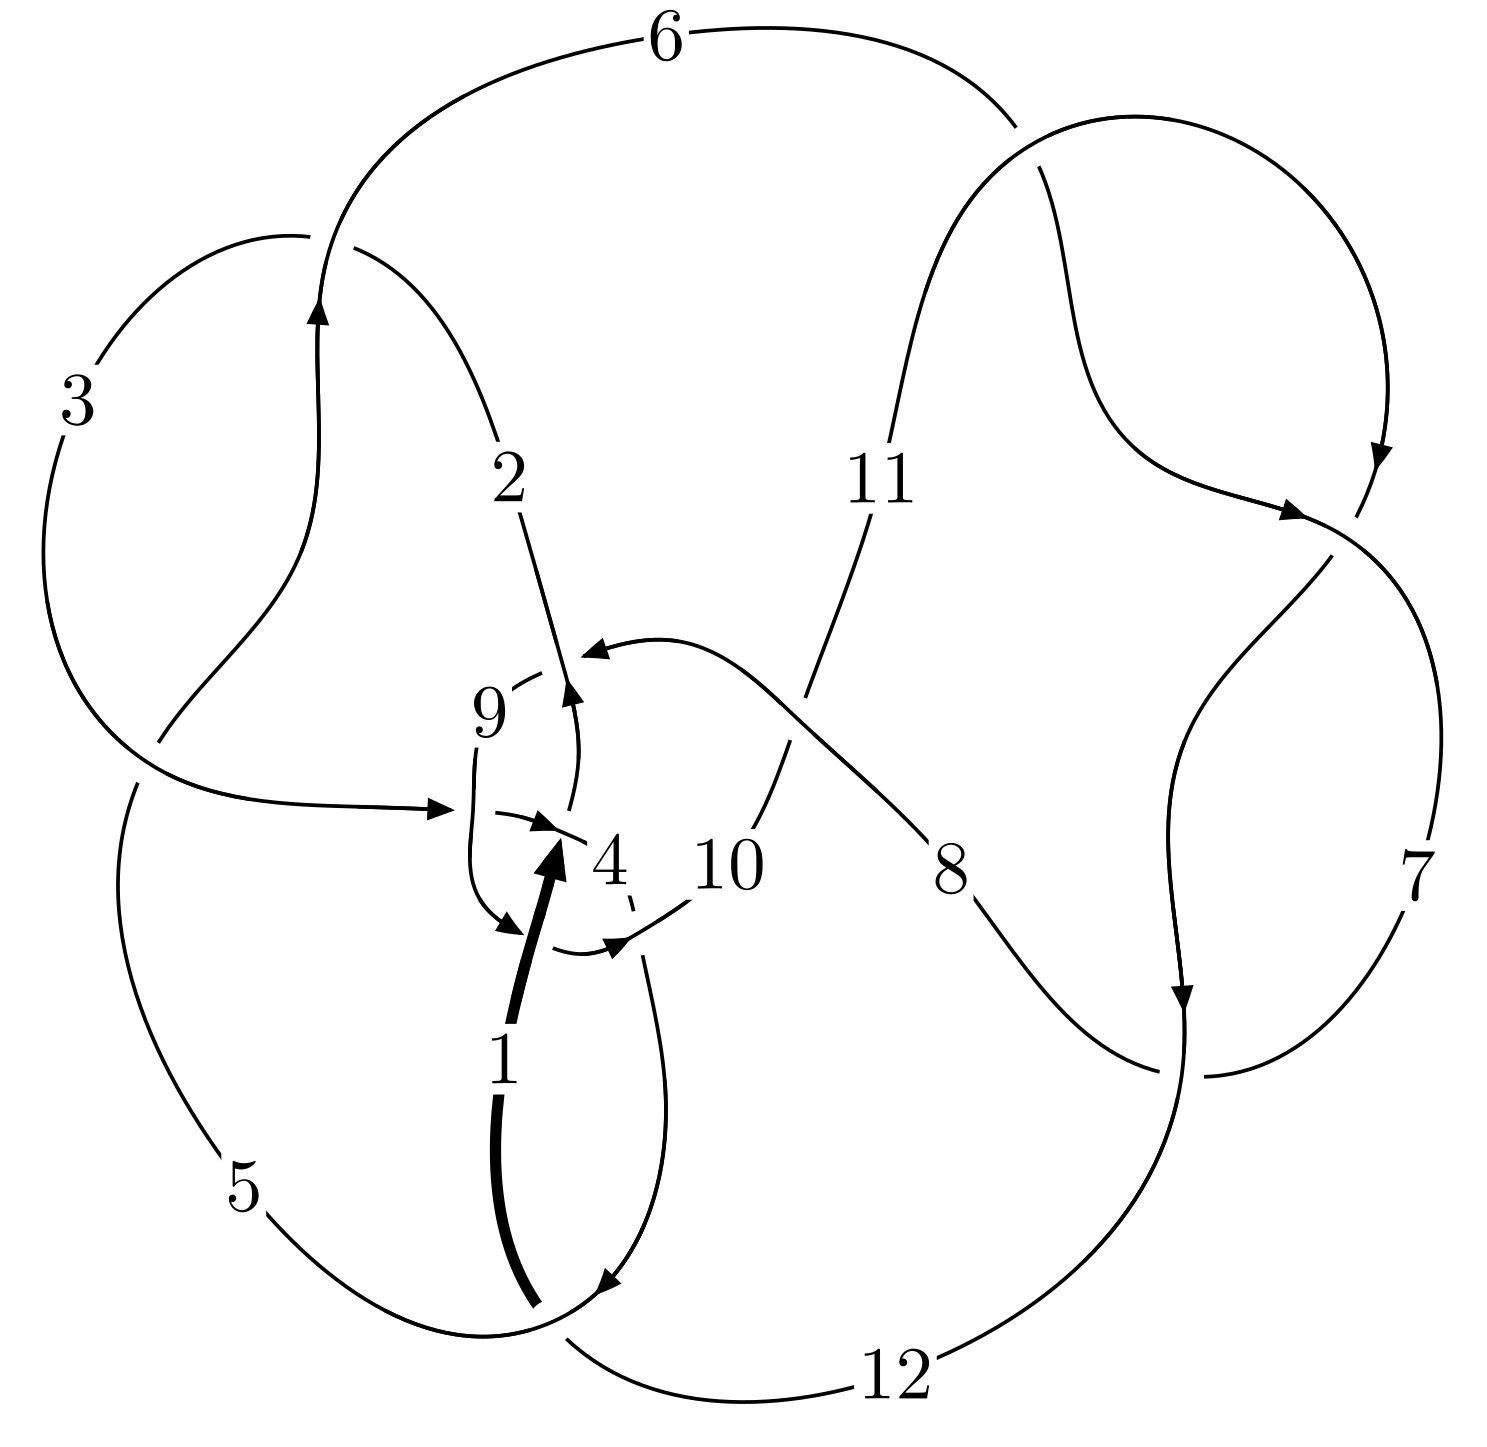
\includegraphics[width=112pt]{../../../GIT/diagram.site/Diagrams/png/1719_12a_0918.png}\\
\ \ \ A knot diagram\footnotemark}&
\allowdisplaybreaks
\textbf{Linearized knot diagam} \\
\cline{2-2}
 &
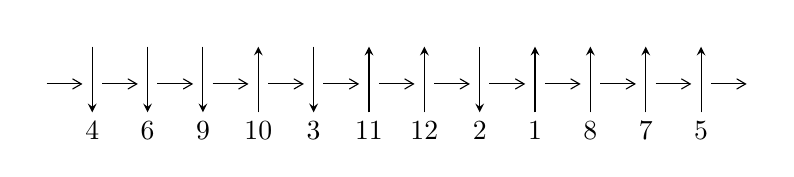
\begin{tikzpicture}[x=20pt, y=17pt]
	% nodes
	\node (C0) at (0, 0) {};
	\node (C1) at (1, 0) {};
	\node (C1U) at (1, +1) {};
	\node (C1D) at (1, -1) {4};

	\node (C2) at (2, 0) {};
	\node (C2U) at (2, +1) {};
	\node (C2D) at (2, -1) {6};

	\node (C3) at (3, 0) {};
	\node (C3U) at (3, +1) {};
	\node (C3D) at (3, -1) {9};

	\node (C4) at (4, 0) {};
	\node (C4U) at (4, +1) {};
	\node (C4D) at (4, -1) {10};

	\node (C5) at (5, 0) {};
	\node (C5U) at (5, +1) {};
	\node (C5D) at (5, -1) {3};

	\node (C6) at (6, 0) {};
	\node (C6U) at (6, +1) {};
	\node (C6D) at (6, -1) {11};

	\node (C7) at (7, 0) {};
	\node (C7U) at (7, +1) {};
	\node (C7D) at (7, -1) {12};

	\node (C8) at (8, 0) {};
	\node (C8U) at (8, +1) {};
	\node (C8D) at (8, -1) {2};

	\node (C9) at (9, 0) {};
	\node (C9U) at (9, +1) {};
	\node (C9D) at (9, -1) {1};

	\node (C10) at (10, 0) {};
	\node (C10U) at (10, +1) {};
	\node (C10D) at (10, -1) {8};

	\node (C11) at (11, 0) {};
	\node (C11U) at (11, +1) {};
	\node (C11D) at (11, -1) {7};

	\node (C12) at (12, 0) {};
	\node (C12U) at (12, +1) {};
	\node (C12D) at (12, -1) {5};
	\node (C13) at (13, 0) {};

	% arrows
	\draw[->,>={angle 60}]
	(C0) edge (C1) (C1) edge (C2) (C2) edge (C3) (C3) edge (C4) (C4) edge (C5) (C5) edge (C6) (C6) edge (C7) (C7) edge (C8) (C8) edge (C9) (C9) edge (C10) (C10) edge (C11) (C11) edge (C12) (C12) edge (C13) ;	\draw[->,>=stealth]
	(C1U) edge (C1D) (C2U) edge (C2D) (C3U) edge (C3D) (C4D) edge (C4U) (C5U) edge (C5D) (C6D) edge (C6U) (C7D) edge (C7U) (C8U) edge (C8D) (C9D) edge (C9U) (C10D) edge (C10U) (C11D) edge (C11U) (C12D) edge (C12U) ;
	\end{tikzpicture} \\
\hhline{~~} \\& 
\textbf{Solving Sequence} \\ \cline{2-2} 
 &
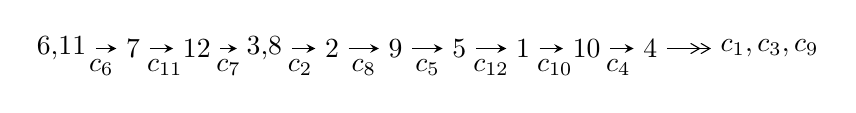
\begin{tikzpicture}[x=23pt, y=7pt]
	% node
	\node (A0) at (-1/8, 0) {6,11};
	\node (A1) at (1, 0) {7};
	\node (A2) at (2, 0) {12};
	\node (A3) at (49/16, 0) {3,8};
	\node (A4) at (33/8, 0) {2};
	\node (A5) at (41/8, 0) {9};
	\node (A6) at (49/8, 0) {5};
	\node (A7) at (57/8, 0) {1};
	\node (A8) at (65/8, 0) {10};
	\node (A9) at (73/8, 0) {4};
	\node (C1) at (1/2, -1) {$c_{6}$};
	\node (C2) at (3/2, -1) {$c_{11}$};
	\node (C3) at (5/2, -1) {$c_{7}$};
	\node (C4) at (29/8, -1) {$c_{2}$};
	\node (C5) at (37/8, -1) {$c_{8}$};
	\node (C6) at (45/8, -1) {$c_{5}$};
	\node (C7) at (53/8, -1) {$c_{12}$};
	\node (C8) at (61/8, -1) {$c_{10}$};
	\node (C9) at (69/8, -1) {$c_{4}$};
	\node (A10) at (11, 0) {$c_{1},c_{3},c_{9}$};

	% edge
	\draw[->,>=stealth]	
	(A0) edge (A1) (A1) edge (A2) (A2) edge (A3) (A3) edge (A4) (A4) edge (A5) (A5) edge (A6) (A6) edge (A7) (A7) edge (A8) (A8) edge (A9) ;
	\draw[->>,>={angle 60}]	
	(A9) edge (A10);
\end{tikzpicture} \\ 

\end{tabular} \\

\footnotetext{
The image of knot diagram is generated by the software ``\textbf{Draw programme}" developed by Andrew Bartholomew(\url{http://www.layer8.co.uk/maths/draw/index.htm\#Running-draw}), where we modified some parts for our purpose(\url{https://github.com/CATsTAILs/LinksPainter}).
}\phantom \\ \newline 
\centering \textbf{Ideals for irreducible components\footnotemark of $X_{\text{par}}$} 
 
\begin{align*}
I^u_{1}&=\langle 
-1.61929\times10^{286} u^{158}+3.80106\times10^{286} u^{157}+\cdots+1.62955\times10^{287} b-5.38191\times10^{287},\\
\phantom{I^u_{1}}&\phantom{= \langle  }2.14088\times10^{287} u^{158}-1.53484\times10^{287} u^{157}+\cdots+5.26470\times10^{287} a+9.88848\times10^{287},\\
\phantom{I^u_{1}}&\phantom{= \langle  }u^{159}+u^{158}+\cdots-92 u+21\rangle \\
I^u_{2}&=\langle 
-20 u^{31}+59 u^{30}+\cdots+b+18,\;15 u^{31}-43 u^{30}+\cdots+a-15,\;u^{32}-4 u^{31}+\cdots+16 u^2+1\rangle \\
I^u_{3}&=\langle 
2 a^3+a^2+b+5 a-3,\;a^4+2 a^2-3 a+1,\;u+1\rangle \\
\\
\end{align*}
\raggedright * 3 irreducible components of $\dim_{\mathbb{C}}=0$, with total 195 representations.\\
\footnotetext{All coefficients of polynomials are rational numbers. But the coefficients are sometimes approximated in decimal forms when there is not enough margin.}
\newpage
\renewcommand{\arraystretch}{1}
\centering \section*{I. $I^u_{1}= \langle -1.62\times10^{286} u^{158}+3.80\times10^{286} u^{157}+\cdots+1.63\times10^{287} b-5.38\times10^{287},\;2.14\times10^{287} u^{158}-1.53\times10^{287} u^{157}+\cdots+5.26\times10^{287} a+9.89\times10^{287},\;u^{159}+u^{158}+\cdots-92 u+21 \rangle$}
\flushleft \textbf{(i) Arc colorings}\\
\begin{tabular}{m{7pt} m{180pt} m{7pt} m{180pt} }
\flushright $a_{6}=$&$\begin{pmatrix}1\\0\end{pmatrix}$ \\
\flushright $a_{11}=$&$\begin{pmatrix}0\\u\end{pmatrix}$ \\
\flushright $a_{7}=$&$\begin{pmatrix}1\\- u^2\end{pmatrix}$ \\
\flushright $a_{12}=$&$\begin{pmatrix}u\\- u^3+u\end{pmatrix}$ \\
\flushright $a_{3}=$&$\begin{pmatrix}-0.406648 u^{158}+0.291533 u^{157}+\cdots-1.00413 u-1.87826\\0.0993705 u^{158}-0.233258 u^{157}+\cdots-19.1997 u+3.30269\end{pmatrix}$ \\
\flushright $a_{8}=$&$\begin{pmatrix}- u^2+1\\u^4-2 u^2\end{pmatrix}$ \\
\flushright $a_{2}=$&$\begin{pmatrix}-0.307277 u^{158}+0.0582749 u^{157}+\cdots-20.2038 u+1.42443\\0.0993705 u^{158}-0.233258 u^{157}+\cdots-19.1997 u+3.30269\end{pmatrix}$ \\
\flushright $a_{9}=$&$\begin{pmatrix}-0.0964387 u^{158}-0.173603 u^{157}+\cdots-78.5154 u+12.5849\\0.305530 u^{158}+0.139750 u^{157}+\cdots+7.38377 u-3.14302\end{pmatrix}$ \\
\flushright $a_{5}=$&$\begin{pmatrix}-0.0972956 u^{158}+0.311974 u^{157}+\cdots+47.8778 u-9.68921\\0.193512 u^{158}-0.201770 u^{157}+\cdots-33.9621 u+9.32314\end{pmatrix}$ \\
\flushright $a_{1}=$&$\begin{pmatrix}0.0386557 u^{158}+0.335671 u^{157}+\cdots+9.26981 u+6.53523\\0.0211241 u^{158}-0.185844 u^{157}+\cdots+9.70779 u-5.49922\end{pmatrix}$ \\
\flushright $a_{10}=$&$\begin{pmatrix}- u^5+2 u^3- u\\u^7-3 u^5+2 u^3+u\end{pmatrix}$ \\
\flushright $a_{4}=$&$\begin{pmatrix}-0.0475849 u^{158}+0.215036 u^{157}+\cdots+49.7268 u-9.69616\\0.197192 u^{158}-0.150861 u^{157}+\cdots-35.7867 u+9.69243\end{pmatrix}$\\&\end{tabular}
\flushleft \textbf{(ii) Obstruction class $= -1$}\\~\\
\flushleft \textbf{(iii) Cusp Shapes $= 0.883281 u^{158}+0.157448 u^{157}+\cdots-191.867 u+45.9615$}\\~\\
\newpage\renewcommand{\arraystretch}{1}
\flushleft \textbf{(iv) u-Polynomials at the component}\newline \\
\begin{tabular}{m{50pt}|m{274pt}}
Crossings & \hspace{64pt}u-Polynomials at each crossing \\
\hline $$\begin{aligned}c_{1}\end{aligned}$$&$\begin{aligned}
&u^{159}-11 u^{158}+\cdots-136 u+48
\end{aligned}$\\
\hline $$\begin{aligned}c_{2},c_{5}\end{aligned}$$&$\begin{aligned}
&u^{159}+9 u^{158}+\cdots+9524 u+1463
\end{aligned}$\\
\hline $$\begin{aligned}c_{3}\end{aligned}$$&$\begin{aligned}
&u^{159}+3 u^{157}+\cdots-349 u-31
\end{aligned}$\\
\hline $$\begin{aligned}c_{4}\end{aligned}$$&$\begin{aligned}
&u^{159}-2 u^{158}+\cdots+576 u-64
\end{aligned}$\\
\hline $$\begin{aligned}c_{6},c_{7},c_{11}\end{aligned}$$&$\begin{aligned}
&u^{159}- u^{158}+\cdots-92 u-21
\end{aligned}$\\
\hline $$\begin{aligned}c_{8}\end{aligned}$$&$\begin{aligned}
&u^{159}-3 u^{158}+\cdots-104013506 u-14233459
\end{aligned}$\\
\hline $$\begin{aligned}c_{9}\end{aligned}$$&$\begin{aligned}
&u^{159}-7 u^{158}+\cdots+113 u-7
\end{aligned}$\\
\hline $$\begin{aligned}c_{10}\end{aligned}$$&$\begin{aligned}
&u^{159}-9 u^{158}+\cdots+3427840 u+1462272
\end{aligned}$\\
\hline $$\begin{aligned}c_{12}\end{aligned}$$&$\begin{aligned}
&u^{159}-3 u^{158}+\cdots+35431 u+1013
\end{aligned}$\\
\hline
\end{tabular}\\~\\
\newpage\renewcommand{\arraystretch}{1}
\flushleft \textbf{(v) Riley Polynomials at the component}\newline \\
\begin{tabular}{m{50pt}|m{274pt}}
Crossings & \hspace{64pt}Riley Polynomials at each crossing \\
\hline $$\begin{aligned}c_{1}\end{aligned}$$&$\begin{aligned}
&y^{159}+3 y^{158}+\cdots-82112 y-2304
\end{aligned}$\\
\hline $$\begin{aligned}c_{2},c_{5}\end{aligned}$$&$\begin{aligned}
&y^{159}+89 y^{158}+\cdots+106035890 y-2140369
\end{aligned}$\\
\hline $$\begin{aligned}c_{3}\end{aligned}$$&$\begin{aligned}
&y^{159}+6 y^{158}+\cdots+80199 y-961
\end{aligned}$\\
\hline $$\begin{aligned}c_{4}\end{aligned}$$&$\begin{aligned}
&y^{159}-2 y^{158}+\cdots+368640 y-4096
\end{aligned}$\\
\hline $$\begin{aligned}c_{6},c_{7},c_{11}\end{aligned}$$&$\begin{aligned}
&y^{159}-147 y^{158}+\cdots-13502 y-441
\end{aligned}$\\
\hline $$\begin{aligned}c_{8}\end{aligned}$$&$\begin{aligned}
&y^{159}+21 y^{158}+\cdots-11556131041417374 y-202591355104681
\end{aligned}$\\
\hline $$\begin{aligned}c_{9}\end{aligned}$$&$\begin{aligned}
&y^{159}+y^{158}+\cdots+4943 y-49
\end{aligned}$\\
\hline $$\begin{aligned}c_{10}\end{aligned}$$&$\begin{aligned}
&y^{159}-3 y^{158}+\cdots-53018876444672 y-2138239401984
\end{aligned}$\\
\hline $$\begin{aligned}c_{12}\end{aligned}$$&$\begin{aligned}
&y^{159}-5 y^{158}+\cdots+327496385 y-1026169
\end{aligned}$\\
\hline
\end{tabular}\\~\\
\newpage\flushleft \textbf{(vi) Complex Volumes and Cusp Shapes}
$$\begin{array}{c|c|c}  
\text{Solutions to }I^u_{1}& \I (\text{vol} + \sqrt{-1}CS) & \text{Cusp shape}\\
 \hline 
\begin{aligned}
u &= -0.799273 + 0.595295 I \\
a &= \phantom{-}0.654341 - 0.752554 I \\
b &= -0.275980 + 1.122700 I\end{aligned}
 & \phantom{-}3.52667 + 1.67894 I & \phantom{-0.000000 } 0 \\ \hline\begin{aligned}
u &= -0.799273 - 0.595295 I \\
a &= \phantom{-}0.654341 + 0.752554 I \\
b &= -0.275980 - 1.122700 I\end{aligned}
 & \phantom{-}3.52667 - 1.67894 I & \phantom{-0.000000 } 0 \\ \hline\begin{aligned}
u &= -0.834666 + 0.572919 I \\
a &= -0.119569 + 0.709332 I \\
b &= \phantom{-}0.401223 - 1.042960 I\end{aligned}
 & \phantom{-}3.33713 + 2.17980 I & \phantom{-0.000000 } 0 \\ \hline\begin{aligned}
u &= -0.834666 - 0.572919 I \\
a &= -0.119569 - 0.709332 I \\
b &= \phantom{-}0.401223 + 1.042960 I\end{aligned}
 & \phantom{-}3.33713 - 2.17980 I & \phantom{-0.000000 } 0 \\ \hline\begin{aligned}
u &= -0.965631 + 0.329670 I \\
a &= \phantom{-}0.760712 - 0.409889 I \\
b &= -0.535440 + 1.145240 I\end{aligned}
 & \phantom{-}1.83061 + 2.86317 I & \phantom{-0.000000 } 0 \\ \hline\begin{aligned}
u &= -0.965631 - 0.329670 I \\
a &= \phantom{-}0.760712 + 0.409889 I \\
b &= -0.535440 - 1.145240 I\end{aligned}
 & \phantom{-}1.83061 - 2.86317 I & \phantom{-0.000000 } 0 \\ \hline\begin{aligned}
u &= \phantom{-}0.788784 + 0.547825 I \\
a &= -0.440608 - 0.644316 I \\
b &= \phantom{-}0.578464 + 1.222480 I\end{aligned}
 & \phantom{-}2.32567 - 11.12500 I & \phantom{-0.000000 } 0 \\ \hline\begin{aligned}
u &= \phantom{-}0.788784 - 0.547825 I \\
a &= -0.440608 + 0.644316 I \\
b &= \phantom{-}0.578464 - 1.222480 I\end{aligned}
 & \phantom{-}2.32567 + 11.12500 I & \phantom{-0.000000 } 0 \\ \hline\begin{aligned}
u &= \phantom{-}0.920641 + 0.229633 I \\
a &= -0.082467 - 1.001120 I \\
b &= \phantom{-}0.673100 + 0.478718 I\end{aligned}
 & -0.75472 + 5.52736 I & \phantom{-0.000000 } 0 \\ \hline\begin{aligned}
u &= \phantom{-}0.920641 - 0.229633 I \\
a &= -0.082467 + 1.001120 I \\
b &= \phantom{-}0.673100 - 0.478718 I\end{aligned}
 & -0.75472 - 5.52736 I & \phantom{-0.000000 } 0\\
 \hline 
 \end{array}$$\newpage$$\begin{array}{c|c|c}  
\text{Solutions to }I^u_{1}& \I (\text{vol} + \sqrt{-1}CS) & \text{Cusp shape}\\
 \hline 
\begin{aligned}
u &= \phantom{-}0.040949 + 0.902867 I \\
a &= \phantom{-}0.164336 + 0.065527 I \\
b &= \phantom{-}0.314215 + 0.827992 I\end{aligned}
 & -2.89952 - 4.98326 I & \phantom{-0.000000 } 0 \\ \hline\begin{aligned}
u &= \phantom{-}0.040949 - 0.902867 I \\
a &= \phantom{-}0.164336 - 0.065527 I \\
b &= \phantom{-}0.314215 - 0.827992 I\end{aligned}
 & -2.89952 + 4.98326 I & \phantom{-0.000000 } 0 \\ \hline\begin{aligned}
u &= \phantom{-}1.088200 + 0.137242 I \\
a &= -0.131931 - 0.931019 I \\
b &= -0.697721 + 0.987501 I\end{aligned}
 & \phantom{-}0.83807 + 4.08830 I & \phantom{-0.000000 } 0 \\ \hline\begin{aligned}
u &= \phantom{-}1.088200 - 0.137242 I \\
a &= -0.131931 + 0.931019 I \\
b &= -0.697721 - 0.987501 I\end{aligned}
 & \phantom{-}0.83807 - 4.08830 I & \phantom{-0.000000 } 0 \\ \hline\begin{aligned}
u &= -0.311564 + 0.832969 I \\
a &= \phantom{-}1.258760 - 0.643598 I \\
b &= \phantom{-}0.498950 + 1.111460 I\end{aligned}
 & \phantom{-}1.69592 - 7.05174 I & \phantom{-0.000000 } 0 \\ \hline\begin{aligned}
u &= -0.311564 - 0.832969 I \\
a &= \phantom{-}1.258760 + 0.643598 I \\
b &= \phantom{-}0.498950 - 1.111460 I\end{aligned}
 & \phantom{-}1.69592 + 7.05174 I & \phantom{-0.000000 } 0 \\ \hline\begin{aligned}
u &= -1.089110 + 0.232449 I \\
a &= \phantom{-}0.69157 + 1.26424 I \\
b &= \phantom{-}0.452532 - 0.926610 I\end{aligned}
 & \phantom{-}0.97576 + 2.58728 I & \phantom{-0.000000 } 0 \\ \hline\begin{aligned}
u &= -1.089110 - 0.232449 I \\
a &= \phantom{-}0.69157 - 1.26424 I \\
b &= \phantom{-}0.452532 + 0.926610 I\end{aligned}
 & \phantom{-}0.97576 - 2.58728 I & \phantom{-0.000000 } 0 \\ \hline\begin{aligned}
u &= -0.334703 + 0.816865 I \\
a &= -0.851963 + 0.666394 I \\
b &= -0.387709 - 1.243550 I\end{aligned}
 & \phantom{-}2.08281 - 6.54231 I & \phantom{-0.000000 } 0 \\ \hline\begin{aligned}
u &= -0.334703 - 0.816865 I \\
a &= -0.851963 - 0.666394 I \\
b &= -0.387709 + 1.243550 I\end{aligned}
 & \phantom{-}2.08281 + 6.54231 I & \phantom{-0.000000 } 0\\
 \hline 
 \end{array}$$\newpage$$\begin{array}{c|c|c}  
\text{Solutions to }I^u_{1}& \I (\text{vol} + \sqrt{-1}CS) & \text{Cusp shape}\\
 \hline 
\begin{aligned}
u &= -1.079580 + 0.301484 I \\
a &= \phantom{-}0.826300 - 0.998104 I \\
b &= \phantom{-}0.314490 + 0.631256 I\end{aligned}
 & \phantom{-}1.81628 - 0.95690 I & \phantom{-0.000000 } 0 \\ \hline\begin{aligned}
u &= -1.079580 - 0.301484 I \\
a &= \phantom{-}0.826300 + 0.998104 I \\
b &= \phantom{-}0.314490 - 0.631256 I\end{aligned}
 & \phantom{-}1.81628 + 0.95690 I & \phantom{-0.000000 } 0 \\ \hline\begin{aligned}
u &= \phantom{-}0.318803 + 0.807507 I \\
a &= \phantom{-}1.30341 + 0.76194 I \\
b &= \phantom{-}0.64770 - 1.28553 I\end{aligned}
 & \phantom{-}0.8176 + 15.8279 I & \phantom{-0.000000 } 0 \\ \hline\begin{aligned}
u &= \phantom{-}0.318803 - 0.807507 I \\
a &= \phantom{-}1.30341 - 0.76194 I \\
b &= \phantom{-}0.64770 + 1.28553 I\end{aligned}
 & \phantom{-}0.8176 - 15.8279 I & \phantom{-0.000000 } 0 \\ \hline\begin{aligned}
u &= \phantom{-}1.164590 + 0.114608 I \\
a &= -0.165064 - 0.937360 I \\
b &= -1.070590 + 0.508490 I\end{aligned}
 & -0.88754 + 2.00188 I & \phantom{-0.000000 } 0 \\ \hline\begin{aligned}
u &= \phantom{-}1.164590 - 0.114608 I \\
a &= -0.165064 + 0.937360 I \\
b &= -1.070590 - 0.508490 I\end{aligned}
 & -0.88754 - 2.00188 I & \phantom{-0.000000 } 0 \\ \hline\begin{aligned}
u &= \phantom{-}1.168020 + 0.107285 I \\
a &= -0.472949 - 0.340663 I \\
b &= -0.135049 - 1.036230 I\end{aligned}
 & \phantom{-}5.53395 - 3.26719 I & \phantom{-0.000000 } 0 \\ \hline\begin{aligned}
u &= \phantom{-}1.168020 - 0.107285 I \\
a &= -0.472949 + 0.340663 I \\
b &= -0.135049 + 1.036230 I\end{aligned}
 & \phantom{-}5.53395 + 3.26719 I & \phantom{-0.000000 } 0 \\ \hline\begin{aligned}
u &= -1.145600 + 0.258752 I \\
a &= \phantom{-}0.469515 + 0.634234 I \\
b &= -0.410048 + 0.042409 I\end{aligned}
 & \phantom{-}0.733678 - 0.678388 I & \phantom{-0.000000 } 0 \\ \hline\begin{aligned}
u &= -1.145600 - 0.258752 I \\
a &= \phantom{-}0.469515 - 0.634234 I \\
b &= -0.410048 - 0.042409 I\end{aligned}
 & \phantom{-}0.733678 + 0.678388 I & \phantom{-0.000000 } 0\\
 \hline 
 \end{array}$$\newpage$$\begin{array}{c|c|c}  
\text{Solutions to }I^u_{1}& \I (\text{vol} + \sqrt{-1}CS) & \text{Cusp shape}\\
 \hline 
\begin{aligned}
u &= \phantom{-}0.767881 + 0.268194 I \\
a &= \phantom{-}0.158187 + 1.260450 I \\
b &= \phantom{-}0.891327 - 0.291243 I\end{aligned}
 & -0.58360 - 5.65390 I & \phantom{-0.000000 } 0 \\ \hline\begin{aligned}
u &= \phantom{-}0.767881 - 0.268194 I \\
a &= \phantom{-}0.158187 - 1.260450 I \\
b &= \phantom{-}0.891327 + 0.291243 I\end{aligned}
 & -0.58360 + 5.65390 I & \phantom{-0.000000 } 0 \\ \hline\begin{aligned}
u &= -1.157610 + 0.341316 I \\
a &= \phantom{-}0.718535 - 0.181945 I \\
b &= \phantom{-}0.336545 + 0.647623 I\end{aligned}
 & \phantom{-}0.097145 - 0.964697 I & \phantom{-0.000000 } 0 \\ \hline\begin{aligned}
u &= -1.157610 - 0.341316 I \\
a &= \phantom{-}0.718535 + 0.181945 I \\
b &= \phantom{-}0.336545 - 0.647623 I\end{aligned}
 & \phantom{-}0.097145 + 0.964697 I & \phantom{-0.000000 } 0 \\ \hline\begin{aligned}
u &= -0.090279 + 0.786792 I \\
a &= \phantom{-}0.310754 - 0.764533 I \\
b &= \phantom{-}0.267372 - 0.570974 I\end{aligned}
 & -3.15929 - 3.12621 I & \phantom{-0.000000 } 0 \\ \hline\begin{aligned}
u &= -0.090279 - 0.786792 I \\
a &= \phantom{-}0.310754 + 0.764533 I \\
b &= \phantom{-}0.267372 + 0.570974 I\end{aligned}
 & -3.15929 + 3.12621 I & \phantom{-0.000000 } 0 \\ \hline\begin{aligned}
u &= -0.211790 + 0.755920 I \\
a &= -1.189780 + 0.211965 I \\
b &= -0.66281 - 1.29058 I\end{aligned}
 & -0.46327 - 6.89398 I & \phantom{-0.000000 } 0 \\ \hline\begin{aligned}
u &= -0.211790 - 0.755920 I \\
a &= -1.189780 - 0.211965 I \\
b &= -0.66281 + 1.29058 I\end{aligned}
 & -0.46327 + 6.89398 I & \phantom{-0.000000 } 0 \\ \hline\begin{aligned}
u &= -0.654320 + 0.409082 I \\
a &= \phantom{-}0.167312 + 0.867181 I \\
b &= -0.242747 - 1.039940 I\end{aligned}
 & \phantom{-}2.56240 - 2.58490 I & \phantom{-}10.69425 + 0. I\phantom{ +0.000000I} \\ \hline\begin{aligned}
u &= -0.654320 - 0.409082 I \\
a &= \phantom{-}0.167312 - 0.867181 I \\
b &= -0.242747 + 1.039940 I\end{aligned}
 & \phantom{-}2.56240 + 2.58490 I & \phantom{-}10.69425 + 0. I\phantom{ +0.000000I}\\
 \hline 
 \end{array}$$\newpage$$\begin{array}{c|c|c}  
\text{Solutions to }I^u_{1}& \I (\text{vol} + \sqrt{-1}CS) & \text{Cusp shape}\\
 \hline 
\begin{aligned}
u &= \phantom{-}0.250992 + 0.726443 I \\
a &= \phantom{-}0.585723 + 0.489535 I \\
b &= \phantom{-}1.153520 + 0.281834 I\end{aligned}
 & -2.37858 + 9.47061 I & \phantom{-0.000000 } 0. - 8.12329 I \\ \hline\begin{aligned}
u &= \phantom{-}0.250992 - 0.726443 I \\
a &= \phantom{-}0.585723 - 0.489535 I \\
b &= \phantom{-}1.153520 - 0.281834 I\end{aligned}
 & -2.37858 - 9.47061 I & \phantom{-0.000000 -}0. + 8.12329 I \\ \hline\begin{aligned}
u &= \phantom{-}0.198555 + 0.737587 I \\
a &= \phantom{-}0.841334 + 0.969239 I \\
b &= \phantom{-}0.407659 - 0.757510 I\end{aligned}
 & -2.98906 - 1.75226 I & \phantom{-0.000000 } 0 \\ \hline\begin{aligned}
u &= \phantom{-}0.198555 - 0.737587 I \\
a &= \phantom{-}0.841334 - 0.969239 I \\
b &= \phantom{-}0.407659 + 0.757510 I\end{aligned}
 & -2.98906 + 1.75226 I & \phantom{-0.000000 } 0 \\ \hline\begin{aligned}
u &= -1.23638\phantom{ +0.000000I} \\
a &= \phantom{-}1.19932\phantom{ +0.000000I} \\
b &= -0.119129\phantom{ +0.000000I}\end{aligned}
 & \phantom{-}2.36933\phantom{ +0.000000I} & \phantom{-0.000000 } 0 \\ \hline\begin{aligned}
u &= \phantom{-}1.152260 + 0.457534 I \\
a &= \phantom{-}0.470420 + 0.899795 I \\
b &= \phantom{-}0.446456 - 0.951171 I\end{aligned}
 & \phantom{-}0.52773 + 9.79628 I & \phantom{-0.000000 } 0 \\ \hline\begin{aligned}
u &= \phantom{-}1.152260 - 0.457534 I \\
a &= \phantom{-}0.470420 - 0.899795 I \\
b &= \phantom{-}0.446456 + 0.951171 I\end{aligned}
 & \phantom{-}0.52773 - 9.79628 I & \phantom{-0.000000 } 0 \\ \hline\begin{aligned}
u &= -1.222050 + 0.211477 I \\
a &= \phantom{-}0.22886 + 1.60032 I \\
b &= -1.076230 - 0.531457 I\end{aligned}
 & -0.21243 - 2.76227 I & \phantom{-0.000000 } 0 \\ \hline\begin{aligned}
u &= -1.222050 - 0.211477 I \\
a &= \phantom{-}0.22886 - 1.60032 I \\
b &= -1.076230 + 0.531457 I\end{aligned}
 & -0.21243 + 2.76227 I & \phantom{-0.000000 } 0 \\ \hline\begin{aligned}
u &= -0.321842 + 0.685356 I \\
a &= \phantom{-}1.44451 - 0.21818 I \\
b &= -0.055055 + 0.871285 I\end{aligned}
 & \phantom{-}1.41713 - 1.34446 I & \phantom{-}6.49984 + 3.60403 I\\
 \hline 
 \end{array}$$\newpage$$\begin{array}{c|c|c}  
\text{Solutions to }I^u_{1}& \I (\text{vol} + \sqrt{-1}CS) & \text{Cusp shape}\\
 \hline 
\begin{aligned}
u &= -0.321842 - 0.685356 I \\
a &= \phantom{-}1.44451 + 0.21818 I \\
b &= -0.055055 - 0.871285 I\end{aligned}
 & \phantom{-}1.41713 + 1.34446 I & \phantom{-}6.49984 - 3.60403 I \\ \hline\begin{aligned}
u &= \phantom{-}0.286131 + 0.695148 I \\
a &= -1.56049 - 0.90920 I \\
b &= -0.65062 + 1.32692 I\end{aligned}
 & -0.20295 + 7.26883 I & -2.50391 - 12.76607 I \\ \hline\begin{aligned}
u &= \phantom{-}0.286131 - 0.695148 I \\
a &= -1.56049 + 0.90920 I \\
b &= -0.65062 - 1.32692 I\end{aligned}
 & -0.20295 - 7.26883 I & -2.50391 + 12.76607 I \\ \hline\begin{aligned}
u &= -0.214279 + 0.711402 I \\
a &= \phantom{-}0.727619 - 0.226998 I \\
b &= \phantom{-}0.619242 - 0.291900 I\end{aligned}
 & -0.67157 - 2.64961 I & \phantom{-}2.00000 + 6.28164 I \\ \hline\begin{aligned}
u &= -0.214279 - 0.711402 I \\
a &= \phantom{-}0.727619 + 0.226998 I \\
b &= \phantom{-}0.619242 + 0.291900 I\end{aligned}
 & -0.67157 + 2.64961 I & \phantom{-}2.00000 - 6.28164 I \\ \hline\begin{aligned}
u &= -0.479596 + 0.566435 I \\
a &= -0.036380 + 0.172804 I \\
b &= \phantom{-}0.436232 - 1.015990 I\end{aligned}
 & \phantom{-}2.36325 - 0.02920 I & \phantom{-}8.14035 + 4.63595 I \\ \hline\begin{aligned}
u &= -0.479596 - 0.566435 I \\
a &= -0.036380 - 0.172804 I \\
b &= \phantom{-}0.436232 + 1.015990 I\end{aligned}
 & \phantom{-}2.36325 + 0.02920 I & \phantom{-}8.14035 - 4.63595 I \\ \hline\begin{aligned}
u &= -0.435949 + 0.572076 I \\
a &= \phantom{-}1.62006 - 0.86038 I \\
b &= \phantom{-}0.585893 + 0.955562 I\end{aligned}
 & \phantom{-}2.27343 - 3.90732 I & \phantom{-}9.31934 + 6.35993 I \\ \hline\begin{aligned}
u &= -0.435949 - 0.572076 I \\
a &= \phantom{-}1.62006 + 0.86038 I \\
b &= \phantom{-}0.585893 - 0.955562 I\end{aligned}
 & \phantom{-}2.27343 + 3.90732 I & \phantom{-}9.31934 - 6.35993 I \\ \hline\begin{aligned}
u &= -0.171511 + 0.685651 I \\
a &= \phantom{-}1.68144 - 1.40388 I \\
b &= \phantom{-}0.336693 + 1.020650 I\end{aligned}
 & -1.71183 - 6.01014 I & -2.05617 + 9.25308 I\\
 \hline 
 \end{array}$$\newpage$$\begin{array}{c|c|c}  
\text{Solutions to }I^u_{1}& \I (\text{vol} + \sqrt{-1}CS) & \text{Cusp shape}\\
 \hline 
\begin{aligned}
u &= -0.171511 - 0.685651 I \\
a &= \phantom{-}1.68144 + 1.40388 I \\
b &= \phantom{-}0.336693 - 1.020650 I\end{aligned}
 & -1.71183 + 6.01014 I & -2.05617 - 9.25308 I \\ \hline\begin{aligned}
u &= -0.130256 + 0.691140 I \\
a &= -0.632396 - 0.435664 I \\
b &= -0.701285 - 0.315380 I\end{aligned}
 & -2.28898 - 2.81780 I & -3.69298 + 6.05931 I \\ \hline\begin{aligned}
u &= -0.130256 - 0.691140 I \\
a &= -0.632396 + 0.435664 I \\
b &= -0.701285 + 0.315380 I\end{aligned}
 & -2.28898 + 2.81780 I & -3.69298 - 6.05931 I \\ \hline\begin{aligned}
u &= \phantom{-}0.364563 + 0.591898 I \\
a &= -0.90629 - 1.42302 I \\
b &= -0.643568 + 0.671849 I\end{aligned}
 & -1.77482 + 3.92949 I & -3.83817 - 8.21365 I \\ \hline\begin{aligned}
u &= \phantom{-}0.364563 - 0.591898 I \\
a &= -0.90629 + 1.42302 I \\
b &= -0.643568 - 0.671849 I\end{aligned}
 & -1.77482 - 3.92949 I & -3.83817 + 8.21365 I \\ \hline\begin{aligned}
u &= -1.232790 + 0.465501 I \\
a &= -0.366440 + 0.564724 I \\
b &= \phantom{-}0.116619 - 0.771707 I\end{aligned}
 & \phantom{-}1.041220 + 0.137927 I & \phantom{-0.000000 } 0 \\ \hline\begin{aligned}
u &= -1.232790 - 0.465501 I \\
a &= -0.366440 - 0.564724 I \\
b &= \phantom{-}0.116619 + 0.771707 I\end{aligned}
 & \phantom{-}1.041220 - 0.137927 I & \phantom{-0.000000 } 0 \\ \hline\begin{aligned}
u &= \phantom{-}0.585666 + 0.340842 I \\
a &= \phantom{-}0.770744 + 0.950438 I \\
b &= -0.528110 - 1.199570 I\end{aligned}
 & \phantom{-}1.10473 - 3.57300 I & \phantom{-}1.47051 + 6.16602 I \\ \hline\begin{aligned}
u &= \phantom{-}0.585666 - 0.340842 I \\
a &= \phantom{-}0.770744 - 0.950438 I \\
b &= -0.528110 + 1.199570 I\end{aligned}
 & \phantom{-}1.10473 + 3.57300 I & \phantom{-}1.47051 - 6.16602 I \\ \hline\begin{aligned}
u &= \phantom{-}0.200680 + 0.637491 I \\
a &= -2.45642 + 0.15855 I \\
b &= -0.313088 + 1.184000 I\end{aligned}
 & \phantom{-}2.97283 + 5.99388 I & \phantom{-}6.42755 - 8.84957 I\\
 \hline 
 \end{array}$$\newpage$$\begin{array}{c|c|c}  
\text{Solutions to }I^u_{1}& \I (\text{vol} + \sqrt{-1}CS) & \text{Cusp shape}\\
 \hline 
\begin{aligned}
u &= \phantom{-}0.200680 - 0.637491 I \\
a &= -2.45642 - 0.15855 I \\
b &= -0.313088 - 1.184000 I\end{aligned}
 & \phantom{-}2.97283 - 5.99388 I & \phantom{-}6.42755 + 8.84957 I \\ \hline\begin{aligned}
u &= \phantom{-}1.336350 + 0.088089 I \\
a &= \phantom{-}0.77234 + 2.29522 I \\
b &= -0.25297 - 1.60145 I\end{aligned}
 & \phantom{-}7.87064 - 3.40592 I & \phantom{-0.000000 } 0 \\ \hline\begin{aligned}
u &= \phantom{-}1.336350 - 0.088089 I \\
a &= \phantom{-}0.77234 - 2.29522 I \\
b &= -0.25297 + 1.60145 I\end{aligned}
 & \phantom{-}7.87064 + 3.40592 I & \phantom{-0.000000 } 0 \\ \hline\begin{aligned}
u &= -1.330760 + 0.168909 I \\
a &= -0.78433 + 2.83863 I \\
b &= -0.425765 - 1.152930 I\end{aligned}
 & \phantom{-}3.75885 - 4.25333 I & \phantom{-0.000000 } 0 \\ \hline\begin{aligned}
u &= -1.330760 - 0.168909 I \\
a &= -0.78433 - 2.83863 I \\
b &= -0.425765 + 1.152930 I\end{aligned}
 & \phantom{-}3.75885 + 4.25333 I & \phantom{-0.000000 } 0 \\ \hline\begin{aligned}
u &= \phantom{-}1.335890 + 0.172092 I \\
a &= \phantom{-}0.075362 + 0.650629 I \\
b &= -0.779588 - 0.974467 I\end{aligned}
 & \phantom{-}3.82140 + 0.23328 I & \phantom{-0.000000 } 0 \\ \hline\begin{aligned}
u &= \phantom{-}1.335890 - 0.172092 I \\
a &= \phantom{-}0.075362 - 0.650629 I \\
b &= -0.779588 + 0.974467 I\end{aligned}
 & \phantom{-}3.82140 - 0.23328 I & \phantom{-0.000000 } 0 \\ \hline\begin{aligned}
u &= \phantom{-}1.337140 + 0.226045 I \\
a &= \phantom{-}0.920513 - 0.672971 I \\
b &= -1.49738 - 0.24928 I\end{aligned}
 & \phantom{-}0.75338 + 3.18644 I & \phantom{-0.000000 } 0 \\ \hline\begin{aligned}
u &= \phantom{-}1.337140 - 0.226045 I \\
a &= \phantom{-}0.920513 + 0.672971 I \\
b &= -1.49738 + 0.24928 I\end{aligned}
 & \phantom{-}0.75338 - 3.18644 I & \phantom{-0.000000 } 0 \\ \hline\begin{aligned}
u &= \phantom{-}0.185771 + 0.615827 I \\
a &= \phantom{-}0.242210 - 0.402152 I \\
b &= -0.674946 - 0.678322 I\end{aligned}
 & -1.75602 - 1.14410 I & -2.70905 + 3.41357 I\\
 \hline 
 \end{array}$$\newpage$$\begin{array}{c|c|c}  
\text{Solutions to }I^u_{1}& \I (\text{vol} + \sqrt{-1}CS) & \text{Cusp shape}\\
 \hline 
\begin{aligned}
u &= \phantom{-}0.185771 - 0.615827 I \\
a &= \phantom{-}0.242210 + 0.402152 I \\
b &= -0.674946 + 0.678322 I\end{aligned}
 & -1.75602 + 1.14410 I & -2.70905 - 3.41357 I \\ \hline\begin{aligned}
u &= \phantom{-}1.320050 + 0.336037 I \\
a &= -0.340469 + 0.295275 I \\
b &= \phantom{-}0.210092 + 0.543789 I\end{aligned}
 & \phantom{-}1.25878 + 7.17293 I & \phantom{-0.000000 } 0 \\ \hline\begin{aligned}
u &= \phantom{-}1.320050 - 0.336037 I \\
a &= -0.340469 - 0.295275 I \\
b &= \phantom{-}0.210092 - 0.543789 I\end{aligned}
 & \phantom{-}1.25878 - 7.17293 I & \phantom{-0.000000 } 0 \\ \hline\begin{aligned}
u &= \phantom{-}1.356050 + 0.157256 I \\
a &= -1.96433 - 2.89991 I \\
b &= -0.070463 + 0.895904 I\end{aligned}
 & \phantom{-}4.84633 - 2.35882 I & \phantom{-0.000000 } 0 \\ \hline\begin{aligned}
u &= \phantom{-}1.356050 - 0.157256 I \\
a &= -1.96433 + 2.89991 I \\
b &= -0.070463 - 0.895904 I\end{aligned}
 & \phantom{-}4.84633 + 2.35882 I & \phantom{-0.000000 } 0 \\ \hline\begin{aligned}
u &= -1.369450 + 0.145280 I \\
a &= -1.036070 + 0.881185 I \\
b &= -0.270195 + 0.271615 I\end{aligned}
 & \phantom{-}4.76561 - 5.98459 I & \phantom{-0.000000 } 0 \\ \hline\begin{aligned}
u &= -1.369450 - 0.145280 I \\
a &= -1.036070 - 0.881185 I \\
b &= -0.270195 - 0.271615 I\end{aligned}
 & \phantom{-}4.76561 + 5.98459 I & \phantom{-0.000000 } 0 \\ \hline\begin{aligned}
u &= \phantom{-}1.351390 + 0.270479 I \\
a &= -0.048448 - 0.646700 I \\
b &= -0.902681 + 0.438862 I\end{aligned}
 & \phantom{-}2.40294 + 6.28854 I & \phantom{-0.000000 } 0 \\ \hline\begin{aligned}
u &= \phantom{-}1.351390 - 0.270479 I \\
a &= -0.048448 + 0.646700 I \\
b &= -0.902681 - 0.438862 I\end{aligned}
 & \phantom{-}2.40294 - 6.28854 I & \phantom{-0.000000 } 0 \\ \hline\begin{aligned}
u &= \phantom{-}0.287478 + 0.545861 I \\
a &= \phantom{-}2.02886 + 0.08096 I \\
b &= \phantom{-}0.331670 - 1.272780 I\end{aligned}
 & \phantom{-}4.08899 - 1.75406 I & \phantom{-}6.02942 - 0.78009 I\\
 \hline 
 \end{array}$$\newpage$$\begin{array}{c|c|c}  
\text{Solutions to }I^u_{1}& \I (\text{vol} + \sqrt{-1}CS) & \text{Cusp shape}\\
 \hline 
\begin{aligned}
u &= \phantom{-}0.287478 - 0.545861 I \\
a &= \phantom{-}2.02886 - 0.08096 I \\
b &= \phantom{-}0.331670 + 1.272780 I\end{aligned}
 & \phantom{-}4.08899 + 1.75406 I & \phantom{-}6.02942 + 0.78009 I \\ \hline\begin{aligned}
u &= -1.368080 + 0.225606 I \\
a &= \phantom{-}1.13965 + 0.97018 I \\
b &= -1.42897 + 0.21580 I\end{aligned}
 & \phantom{-}1.13488 - 3.60883 I & \phantom{-0.000000 } 0 \\ \hline\begin{aligned}
u &= -1.368080 - 0.225606 I \\
a &= \phantom{-}1.13965 - 0.97018 I \\
b &= -1.42897 - 0.21580 I\end{aligned}
 & \phantom{-}1.13488 + 3.60883 I & \phantom{-0.000000 } 0 \\ \hline\begin{aligned}
u &= \phantom{-}0.156361 + 0.590337 I \\
a &= -0.909143 - 1.010760 I \\
b &= -1.254360 - 0.266293 I\end{aligned}
 & -3.73265 + 0.64583 I & -14.3996 - 3.2867 I \\ \hline\begin{aligned}
u &= \phantom{-}0.156361 - 0.590337 I \\
a &= -0.909143 + 1.010760 I \\
b &= -1.254360 + 0.266293 I\end{aligned}
 & -3.73265 - 0.64583 I & -14.3996 + 3.2867 I \\ \hline\begin{aligned}
u &= -1.382100 + 0.159658 I \\
a &= \phantom{-}0.40621 - 2.75500 I \\
b &= -0.27264 + 1.41868 I\end{aligned}
 & \phantom{-}9.38761 + 1.59220 I & \phantom{-0.000000 } 0 \\ \hline\begin{aligned}
u &= -1.382100 - 0.159658 I \\
a &= \phantom{-}0.40621 + 2.75500 I \\
b &= -0.27264 - 1.41868 I\end{aligned}
 & \phantom{-}9.38761 - 1.59220 I & \phantom{-0.000000 } 0 \\ \hline\begin{aligned}
u &= -0.072608 + 0.602082 I \\
a &= -1.253030 + 0.070063 I \\
b &= -1.283910 + 0.307868 I\end{aligned}
 & -3.72634 - 0.20894 I & -8.98173 - 0.59922 I \\ \hline\begin{aligned}
u &= -0.072608 - 0.602082 I \\
a &= -1.253030 - 0.070063 I \\
b &= -1.283910 - 0.307868 I\end{aligned}
 & -3.72634 + 0.20894 I & -8.98173 + 0.59922 I \\ \hline\begin{aligned}
u &= \phantom{-}1.369520 + 0.270922 I \\
a &= \phantom{-}1.21441 + 2.78141 I \\
b &= \phantom{-}0.269286 - 1.108730 I\end{aligned}
 & \phantom{-}3.18591 + 9.47700 I & \phantom{-0.000000 } 0\\
 \hline 
 \end{array}$$\newpage$$\begin{array}{c|c|c}  
\text{Solutions to }I^u_{1}& \I (\text{vol} + \sqrt{-1}CS) & \text{Cusp shape}\\
 \hline 
\begin{aligned}
u &= \phantom{-}1.369520 - 0.270922 I \\
a &= \phantom{-}1.21441 - 2.78141 I \\
b &= \phantom{-}0.269286 + 1.108730 I\end{aligned}
 & \phantom{-}3.18591 - 9.47700 I & \phantom{-0.000000 } 0 \\ \hline\begin{aligned}
u &= -1.365110 + 0.295551 I \\
a &= \phantom{-}0.82503 - 1.91460 I \\
b &= \phantom{-}0.271144 + 0.950814 I\end{aligned}
 & \phantom{-}1.94770 - 1.99435 I & \phantom{-0.000000 } 0 \\ \hline\begin{aligned}
u &= -1.365110 - 0.295551 I \\
a &= \phantom{-}0.82503 + 1.91460 I \\
b &= \phantom{-}0.271144 - 0.950814 I\end{aligned}
 & \phantom{-}1.94770 + 1.99435 I & \phantom{-0.000000 } 0 \\ \hline\begin{aligned}
u &= \phantom{-}1.396810 + 0.099721 I \\
a &= -0.176525 - 0.092513 I \\
b &= \phantom{-}0.612241 + 0.391261 I\end{aligned}
 & \phantom{-}6.97211 + 1.72636 I & \phantom{-0.000000 } 0 \\ \hline\begin{aligned}
u &= \phantom{-}1.396810 - 0.099721 I \\
a &= -0.176525 + 0.092513 I \\
b &= \phantom{-}0.612241 - 0.391261 I\end{aligned}
 & \phantom{-}6.97211 - 1.72636 I & \phantom{-0.000000 } 0 \\ \hline\begin{aligned}
u &= -1.379490 + 0.256508 I \\
a &= -1.88048 + 1.78681 I \\
b &= -0.403089 - 1.223300 I\end{aligned}
 & \phantom{-}8.00556 - 9.26916 I & \phantom{-0.000000 } 0 \\ \hline\begin{aligned}
u &= -1.379490 - 0.256508 I \\
a &= -1.88048 - 1.78681 I \\
b &= -0.403089 + 1.223300 I\end{aligned}
 & \phantom{-}8.00556 + 9.26916 I & \phantom{-0.000000 } 0 \\ \hline\begin{aligned}
u &= -1.403520 + 0.086431 I \\
a &= -0.497455 - 0.628849 I \\
b &= \phantom{-}0.981614 - 0.222678 I\end{aligned}
 & \phantom{-}5.71530 + 4.79848 I & \phantom{-0.000000 } 0 \\ \hline\begin{aligned}
u &= -1.403520 - 0.086431 I \\
a &= -0.497455 + 0.628849 I \\
b &= \phantom{-}0.981614 + 0.222678 I\end{aligned}
 & \phantom{-}5.71530 - 4.79848 I & \phantom{-0.000000 } 0 \\ \hline\begin{aligned}
u &= -1.391830 + 0.201064 I \\
a &= -0.93217 + 2.23738 I \\
b &= \phantom{-}0.22876 - 1.66694 I\end{aligned}
 & \phantom{-}9.66378 - 7.08739 I & \phantom{-0.000000 } 0\\
 \hline 
 \end{array}$$\newpage$$\begin{array}{c|c|c}  
\text{Solutions to }I^u_{1}& \I (\text{vol} + \sqrt{-1}CS) & \text{Cusp shape}\\
 \hline 
\begin{aligned}
u &= -1.391830 - 0.201064 I \\
a &= -0.93217 - 2.23738 I \\
b &= \phantom{-}0.22876 + 1.66694 I\end{aligned}
 & \phantom{-}9.66378 + 7.08739 I & \phantom{-0.000000 } 0 \\ \hline\begin{aligned}
u &= -1.386000 + 0.246655 I \\
a &= \phantom{-}0.921726 - 0.266770 I \\
b &= -0.785839 + 0.498129 I\end{aligned}
 & \phantom{-}3.30331 - 2.00372 I & \phantom{-0.000000 } 0 \\ \hline\begin{aligned}
u &= -1.386000 - 0.246655 I \\
a &= \phantom{-}0.921726 + 0.266770 I \\
b &= -0.785839 - 0.498129 I\end{aligned}
 & \phantom{-}3.30331 + 2.00372 I & \phantom{-0.000000 } 0 \\ \hline\begin{aligned}
u &= -1.39993 + 0.21353 I \\
a &= \phantom{-}1.17608 - 2.01178 I \\
b &= \phantom{-}0.50864 + 1.36234 I\end{aligned}
 & \phantom{-}9.46503 - 1.05151 I & \phantom{-0.000000 } 0 \\ \hline\begin{aligned}
u &= -1.39993 - 0.21353 I \\
a &= \phantom{-}1.17608 + 2.01178 I \\
b &= \phantom{-}0.50864 - 1.36234 I\end{aligned}
 & \phantom{-}9.46503 + 1.05151 I & \phantom{-0.000000 } 0 \\ \hline\begin{aligned}
u &= \phantom{-}1.38973 + 0.28573 I \\
a &= -0.215171 + 0.305291 I \\
b &= \phantom{-}0.803425 + 0.224199 I\end{aligned}
 & \phantom{-}4.43971 + 6.27448 I & \phantom{-0.000000 } 0 \\ \hline\begin{aligned}
u &= \phantom{-}1.38973 - 0.28573 I \\
a &= -0.215171 - 0.305291 I \\
b &= \phantom{-}0.803425 - 0.224199 I\end{aligned}
 & \phantom{-}4.43971 - 6.27448 I & \phantom{-0.000000 } 0 \\ \hline\begin{aligned}
u &= \phantom{-}1.38660 + 0.30322 I \\
a &= -0.90903 - 2.01619 I \\
b &= -0.71453 + 1.39926 I\end{aligned}
 & \phantom{-}4.61255 + 10.72160 I & \phantom{-0.000000 } 0 \\ \hline\begin{aligned}
u &= \phantom{-}1.38660 - 0.30322 I \\
a &= -0.90903 + 2.01619 I \\
b &= -0.71453 - 1.39926 I\end{aligned}
 & \phantom{-}4.61255 - 10.72160 I & \phantom{-0.000000 } 0 \\ \hline\begin{aligned}
u &= \phantom{-}1.41466 + 0.12761 I \\
a &= \phantom{-}0.25482 - 2.27671 I \\
b &= -0.071824 + 1.276080 I\end{aligned}
 & \phantom{-}8.86441 + 4.13680 I & \phantom{-0.000000 } 0\\
 \hline 
 \end{array}$$\newpage$$\begin{array}{c|c|c}  
\text{Solutions to }I^u_{1}& \I (\text{vol} + \sqrt{-1}CS) & \text{Cusp shape}\\
 \hline 
\begin{aligned}
u &= \phantom{-}1.41466 - 0.12761 I \\
a &= \phantom{-}0.25482 + 2.27671 I \\
b &= -0.071824 - 1.276080 I\end{aligned}
 & \phantom{-}8.86441 - 4.13680 I & \phantom{-0.000000 } 0 \\ \hline\begin{aligned}
u &= -1.40230 + 0.28947 I \\
a &= -0.799094 - 0.602129 I \\
b &= \phantom{-}1.269700 - 0.233757 I\end{aligned}
 & \phantom{-}2.88682 - 13.15910 I & \phantom{-0.000000 } 0 \\ \hline\begin{aligned}
u &= -1.40230 - 0.28947 I \\
a &= -0.799094 + 0.602129 I \\
b &= \phantom{-}1.269700 + 0.233757 I\end{aligned}
 & \phantom{-}2.88682 + 13.15910 I & \phantom{-0.000000 } 0 \\ \hline\begin{aligned}
u &= -1.42930 + 0.12679 I \\
a &= \phantom{-}0.99232 - 2.26659 I \\
b &= -0.355357 + 1.353570 I\end{aligned}
 & \phantom{-}7.30600 + 1.91757 I & \phantom{-0.000000 } 0 \\ \hline\begin{aligned}
u &= -1.42930 - 0.12679 I \\
a &= \phantom{-}0.99232 + 2.26659 I \\
b &= -0.355357 - 1.353570 I\end{aligned}
 & \phantom{-}7.30600 - 1.91757 I & \phantom{-0.000000 } 0 \\ \hline\begin{aligned}
u &= -1.41558 + 0.27321 I \\
a &= -0.99899 + 2.49915 I \\
b &= -0.66005 - 1.41457 I\end{aligned}
 & \phantom{-}5.23264 - 10.79800 I & \phantom{-0.000000 } 0 \\ \hline\begin{aligned}
u &= -1.41558 - 0.27321 I \\
a &= -0.99899 - 2.49915 I \\
b &= -0.66005 + 1.41457 I\end{aligned}
 & \phantom{-}5.23264 + 10.79800 I & \phantom{-0.000000 } 0 \\ \hline\begin{aligned}
u &= \phantom{-}1.42343 + 0.26174 I \\
a &= \phantom{-}1.41395 + 1.31316 I \\
b &= \phantom{-}0.103083 - 0.897993 I\end{aligned}
 & \phantom{-}6.99165 + 4.78322 I & \phantom{-0.000000 } 0 \\ \hline\begin{aligned}
u &= \phantom{-}1.42343 - 0.26174 I \\
a &= \phantom{-}1.41395 - 1.31316 I \\
b &= \phantom{-}0.103083 + 0.897993 I\end{aligned}
 & \phantom{-}6.99165 - 4.78322 I & \phantom{-0.000000 } 0 \\ \hline\begin{aligned}
u &= \phantom{-}1.43411 + 0.20911 I \\
a &= \phantom{-}0.73448 + 1.85336 I \\
b &= \phantom{-}0.724979 - 1.032690 I\end{aligned}
 & \phantom{-}8.20112 + 6.72484 I & \phantom{-0.000000 } 0\\
 \hline 
 \end{array}$$\newpage$$\begin{array}{c|c|c}  
\text{Solutions to }I^u_{1}& \I (\text{vol} + \sqrt{-1}CS) & \text{Cusp shape}\\
 \hline 
\begin{aligned}
u &= \phantom{-}1.43411 - 0.20911 I \\
a &= \phantom{-}0.73448 - 1.85336 I \\
b &= \phantom{-}0.724979 + 1.032690 I\end{aligned}
 & \phantom{-}8.20112 - 6.72484 I & \phantom{-0.000000 } 0 \\ \hline\begin{aligned}
u &= -0.498633 + 0.231913 I \\
a &= \phantom{-}0.676707 - 0.369974 I \\
b &= \phantom{-}0.235110 - 0.126078 I\end{aligned}
 & \phantom{-}1.125340 - 0.507072 I & \phantom{-}7.32472 + 1.80737 I \\ \hline\begin{aligned}
u &= -0.498633 - 0.231913 I \\
a &= \phantom{-}0.676707 + 0.369974 I \\
b &= \phantom{-}0.235110 + 0.126078 I\end{aligned}
 & \phantom{-}1.125340 + 0.507072 I & \phantom{-}7.32472 - 1.80737 I \\ \hline\begin{aligned}
u &= \phantom{-}1.44415 + 0.18611 I \\
a &= -0.50108 - 1.52574 I \\
b &= \phantom{-}0.395517 + 1.192830 I\end{aligned}
 & \phantom{-}8.50916 + 2.66886 I & \phantom{-0.000000 } 0 \\ \hline\begin{aligned}
u &= \phantom{-}1.44415 - 0.18611 I \\
a &= -0.50108 + 1.52574 I \\
b &= \phantom{-}0.395517 - 1.192830 I\end{aligned}
 & \phantom{-}8.50916 - 2.66886 I & \phantom{-0.000000 } 0 \\ \hline\begin{aligned}
u &= \phantom{-}0.265097 + 0.456539 I \\
a &= -0.609248 - 0.288943 I \\
b &= \phantom{-}0.10567 + 1.51534 I\end{aligned}
 & \phantom{-}4.39118 + 4.54039 I & \phantom{-}5.47207 - 10.36562 I \\ \hline\begin{aligned}
u &= \phantom{-}0.265097 - 0.456539 I \\
a &= -0.609248 + 0.288943 I \\
b &= \phantom{-}0.10567 - 1.51534 I\end{aligned}
 & \phantom{-}4.39118 - 4.54039 I & \phantom{-}5.47207 + 10.36562 I \\ \hline\begin{aligned}
u &= -1.44253 + 0.32040 I \\
a &= \phantom{-}0.95994 - 2.16725 I \\
b &= \phantom{-}0.66728 + 1.34561 I\end{aligned}
 & \phantom{-}6.4467 - 19.9152 I & \phantom{-0.000000 } 0 \\ \hline\begin{aligned}
u &= -1.44253 - 0.32040 I \\
a &= \phantom{-}0.95994 + 2.16725 I \\
b &= \phantom{-}0.66728 - 1.34561 I\end{aligned}
 & \phantom{-}6.4467 + 19.9152 I & \phantom{-0.000000 } 0 \\ \hline\begin{aligned}
u &= \phantom{-}1.44201 + 0.33238 I \\
a &= \phantom{-}1.04232 + 1.86273 I \\
b &= \phantom{-}0.538860 - 1.182240 I\end{aligned}
 & \phantom{-}7.29386 + 11.26600 I & \phantom{-0.000000 } 0\\
 \hline 
 \end{array}$$\newpage$$\begin{array}{c|c|c}  
\text{Solutions to }I^u_{1}& \I (\text{vol} + \sqrt{-1}CS) & \text{Cusp shape}\\
 \hline 
\begin{aligned}
u &= \phantom{-}1.44201 - 0.33238 I \\
a &= \phantom{-}1.04232 - 1.86273 I \\
b &= \phantom{-}0.538860 + 1.182240 I\end{aligned}
 & \phantom{-}7.29386 - 11.26600 I & \phantom{-0.000000 } 0 \\ \hline\begin{aligned}
u &= \phantom{-}1.44792 + 0.32031 I \\
a &= -0.83095 - 2.00003 I \\
b &= -0.403517 + 1.354990 I\end{aligned}
 & \phantom{-}7.78199 + 10.65610 I & \phantom{-0.000000 } 0 \\ \hline\begin{aligned}
u &= \phantom{-}1.44792 - 0.32031 I \\
a &= -0.83095 + 2.00003 I \\
b &= -0.403517 - 1.354990 I\end{aligned}
 & \phantom{-}7.78199 - 10.65610 I & \phantom{-0.000000 } 0 \\ \hline\begin{aligned}
u &= -1.46623 + 0.22801 I \\
a &= -0.35046 + 2.00234 I \\
b &= -0.520060 - 0.833912 I\end{aligned}
 & \phantom{-}4.17918 - 6.96018 I & \phantom{-0.000000 } 0 \\ \hline\begin{aligned}
u &= -1.46623 - 0.22801 I \\
a &= -0.35046 - 2.00234 I \\
b &= -0.520060 + 0.833912 I\end{aligned}
 & \phantom{-}4.17918 + 6.96018 I & \phantom{-0.000000 } 0 \\ \hline\begin{aligned}
u &= -1.54158 + 0.06730 I \\
a &= -0.48637 + 1.93480 I \\
b &= \phantom{-}0.423099 - 1.272070 I\end{aligned}
 & \phantom{-}10.20780 + 9.30854 I & \phantom{-0.000000 } 0 \\ \hline\begin{aligned}
u &= -1.54158 - 0.06730 I \\
a &= -0.48637 - 1.93480 I \\
b &= \phantom{-}0.423099 + 1.272070 I\end{aligned}
 & \phantom{-}10.20780 - 9.30854 I & \phantom{-0.000000 } 0 \\ \hline\begin{aligned}
u &= -0.005487 + 0.448891 I \\
a &= -2.54974 - 0.62221 I \\
b &= -0.568904 + 0.992243 I\end{aligned}
 & -0.54033 + 2.01867 I & -2.68262 - 3.08744 I \\ \hline\begin{aligned}
u &= -0.005487 - 0.448891 I \\
a &= -2.54974 + 0.62221 I \\
b &= -0.568904 - 0.992243 I\end{aligned}
 & -0.54033 - 2.01867 I & -2.68262 + 3.08744 I \\ \hline\begin{aligned}
u &= \phantom{-}1.58971 + 0.03349 I \\
a &= \phantom{-}0.19891 + 1.82666 I \\
b &= \phantom{-}0.022223 - 1.145830 I\end{aligned}
 & \phantom{-}11.83510 + 0.31664 I & \phantom{-0.000000 } 0\\
 \hline 
 \end{array}$$\newpage$$\begin{array}{c|c|c}  
\text{Solutions to }I^u_{1}& \I (\text{vol} + \sqrt{-1}CS) & \text{Cusp shape}\\
 \hline 
\begin{aligned}
u &= \phantom{-}1.58971 - 0.03349 I \\
a &= \phantom{-}0.19891 - 1.82666 I \\
b &= \phantom{-}0.022223 + 1.145830 I\end{aligned}
 & \phantom{-}11.83510 - 0.31664 I & \phantom{-0.000000 } 0 \\ \hline\begin{aligned}
u &= \phantom{-}0.233535 + 0.310327 I \\
a &= \phantom{-}0.01580 + 1.99878 I \\
b &= -0.192951 - 1.356770 I\end{aligned}
 & \phantom{-}4.22259 - 3.55617 I & \phantom{-}11.75571 - 4.38189 I \\ \hline\begin{aligned}
u &= \phantom{-}0.233535 - 0.310327 I \\
a &= \phantom{-}0.01580 - 1.99878 I \\
b &= -0.192951 + 1.356770 I\end{aligned}
 & \phantom{-}4.22259 + 3.55617 I & \phantom{-}11.75571 + 4.38189 I \\ \hline\begin{aligned}
u &= \phantom{-}0.281817 + 0.265812 I \\
a &= \phantom{-}1.043980 + 0.163916 I \\
b &= -0.629326 - 0.360289 I\end{aligned}
 & -1.37561 - 0.94145 I & -2.52295 + 1.00632 I \\ \hline\begin{aligned}
u &= \phantom{-}0.281817 - 0.265812 I \\
a &= \phantom{-}1.043980 - 0.163916 I \\
b &= -0.629326 + 0.360289 I\end{aligned}
 & -1.37561 + 0.94145 I & -2.52295 - 1.00632 I \\ \hline\begin{aligned}
u &= \phantom{-}1.61353 + 0.03083 I \\
a &= \phantom{-}0.01106 - 1.76492 I \\
b &= \phantom{-}0.135699 + 1.074040 I\end{aligned}
 & \phantom{-}11.79000 - 0.33406 I & \phantom{-0.000000 } 0 \\ \hline\begin{aligned}
u &= \phantom{-}1.61353 - 0.03083 I \\
a &= \phantom{-}0.01106 + 1.76492 I \\
b &= \phantom{-}0.135699 - 1.074040 I\end{aligned}
 & \phantom{-}11.79000 + 0.33406 I & \phantom{-0.000000 } 0 \\ \hline\begin{aligned}
u &= -0.044735 + 0.337560 I \\
a &= -6.29736 + 0.56249 I \\
b &= \phantom{-}0.048607 - 0.637881 I\end{aligned}
 & \phantom{-}0.20790 + 4.29893 I & \phantom{-}2.06844 + 3.27592 I \\ \hline\begin{aligned}
u &= -0.044735 - 0.337560 I \\
a &= -6.29736 - 0.56249 I \\
b &= \phantom{-}0.048607 + 0.637881 I\end{aligned}
 & \phantom{-}0.20790 - 4.29893 I & \phantom{-}2.06844 - 3.27592 I\\
 \hline 
 \end{array}$$\newpage\newpage\renewcommand{\arraystretch}{1}
\centering \section*{II. $I^u_{2}= \langle -20 u^{31}+59 u^{30}+\cdots+b+18,\;15 u^{31}-43 u^{30}+\cdots+a-15,\;u^{32}-4 u^{31}+\cdots+16 u^2+1 \rangle$}
\flushleft \textbf{(i) Arc colorings}\\
\begin{tabular}{m{7pt} m{180pt} m{7pt} m{180pt} }
\flushright $a_{6}=$&$\begin{pmatrix}1\\0\end{pmatrix}$ \\
\flushright $a_{11}=$&$\begin{pmatrix}0\\u\end{pmatrix}$ \\
\flushright $a_{7}=$&$\begin{pmatrix}1\\- u^2\end{pmatrix}$ \\
\flushright $a_{12}=$&$\begin{pmatrix}u\\- u^3+u\end{pmatrix}$ \\
\flushright $a_{3}=$&$\begin{pmatrix}-15 u^{31}+43 u^{30}+\cdots+3 u+15\\20 u^{31}-59 u^{30}+\cdots-9 u-18\end{pmatrix}$ \\
\flushright $a_{8}=$&$\begin{pmatrix}- u^2+1\\u^4-2 u^2\end{pmatrix}$ \\
\flushright $a_{2}=$&$\begin{pmatrix}5 u^{31}-16 u^{30}+\cdots-6 u-3\\20 u^{31}-59 u^{30}+\cdots-9 u-18\end{pmatrix}$ \\
\flushright $a_{9}=$&$\begin{pmatrix}50 u^{31}-135 u^{30}+\cdots-11 u-38\\-12 u^{31}+27 u^{30}+\cdots-3 u+4\end{pmatrix}$ \\
\flushright $a_{5}=$&$\begin{pmatrix}20 u^{31}-40 u^{30}+\cdots-14 u-7\\-20 u^{31}+46 u^{30}+\cdots+9 u+14\end{pmatrix}$ \\
\flushright $a_{1}=$&$\begin{pmatrix}40 u^{31}-104 u^{30}+\cdots-41 u-32\\-32 u^{31}+82 u^{30}+\cdots+17 u+25\end{pmatrix}$ \\
\flushright $a_{10}=$&$\begin{pmatrix}- u^5+2 u^3- u\\u^7-3 u^5+2 u^3+u\end{pmatrix}$ \\
\flushright $a_{4}=$&$\begin{pmatrix}2 u^{31}+4 u^{30}+\cdots-7 u+5\\- u^{31}-2 u^{30}+\cdots+u+1\end{pmatrix}$\\&\end{tabular}
\flushleft \textbf{(ii) Obstruction class $= 1$}\\~\\
\flushleft \textbf{(iii) Cusp Shapes $= -131 u^{31}+354 u^{30}+1641 u^{29}-4684 u^{28}-9391 u^{27}+27382 u^{26}+33163 u^{25}-91574 u^{24}-82869 u^{23}+186844 u^{22}+157052 u^{21}-218430 u^{20}-224559 u^{19}+81246 u^{18}+216620 u^{17}+149426 u^{16}-90371 u^{15}-233798 u^{14}-67401 u^{13}+96549 u^{12}+108708 u^{11}+51286 u^{10}-39137 u^9-53047 u^8-10210 u^7+1070 u^6+6176 u^5+6250 u^4+450 u^3+1554 u^2+34 u+90$}\\~\\
\newpage\renewcommand{\arraystretch}{1}
\flushleft \textbf{(iv) u-Polynomials at the component}\newline \\
\begin{tabular}{m{50pt}|m{274pt}}
Crossings & \hspace{64pt}u-Polynomials at each crossing \\
\hline $$\begin{aligned}c_{1}\end{aligned}$$&$\begin{aligned}
&u^{32}-6 u^{31}+\cdots-27 u+13
\end{aligned}$\\
\hline $$\begin{aligned}c_{2}\end{aligned}$$&$\begin{aligned}
&u^{32}-10 u^{31}+\cdots-4 u+1
\end{aligned}$\\
\hline $$\begin{aligned}c_{3}\end{aligned}$$&$\begin{aligned}
&u^{32}+7 u^{30}+\cdots+7 u^2+1
\end{aligned}$\\
\hline $$\begin{aligned}c_{4}\end{aligned}$$&$\begin{aligned}
&u^{32}+7 u^{30}+\cdots+7 u^2+1
\end{aligned}$\\
\hline $$\begin{aligned}c_{5}\end{aligned}$$&$\begin{aligned}
&u^{32}+10 u^{31}+\cdots+4 u+1
\end{aligned}$\\
\hline $$\begin{aligned}c_{6},c_{7}\end{aligned}$$&$\begin{aligned}
&u^{32}-4 u^{31}+\cdots+16 u^2+1
\end{aligned}$\\
\hline $$\begin{aligned}c_{8}\end{aligned}$$&$\begin{aligned}
&u^{32}-5 u^{30}+\cdots+31 u+11
\end{aligned}$\\
\hline $$\begin{aligned}c_{9}\end{aligned}$$&$\begin{aligned}
&u^{32}-2 u^{31}+\cdots+4 u^2+1
\end{aligned}$\\
\hline $$\begin{aligned}c_{10}\end{aligned}$$&$\begin{aligned}
&u^{32}-12 u^{31}+\cdots-60 u+13
\end{aligned}$\\
\hline $$\begin{aligned}c_{11}\end{aligned}$$&$\begin{aligned}
&u^{32}+4 u^{31}+\cdots+16 u^2+1
\end{aligned}$\\
\hline $$\begin{aligned}c_{12}\end{aligned}$$&$\begin{aligned}
&u^{32}-2 u^{31}+\cdots+19 u+11
\end{aligned}$\\
\hline
\end{tabular}\\~\\
\newpage\renewcommand{\arraystretch}{1}
\flushleft \textbf{(v) Riley Polynomials at the component}\newline \\
\begin{tabular}{m{50pt}|m{274pt}}
Crossings & \hspace{64pt}Riley Polynomials at each crossing \\
\hline $$\begin{aligned}c_{1}\end{aligned}$$&$\begin{aligned}
&y^{32}-12 y^{31}+\cdots-1145 y+169
\end{aligned}$\\
\hline $$\begin{aligned}c_{2},c_{5}\end{aligned}$$&$\begin{aligned}
&y^{32}+16 y^{31}+\cdots+30 y+1
\end{aligned}$\\
\hline $$\begin{aligned}c_{3}\end{aligned}$$&$\begin{aligned}
&y^{32}+14 y^{31}+\cdots+14 y+1
\end{aligned}$\\
\hline $$\begin{aligned}c_{4}\end{aligned}$$&$\begin{aligned}
&y^{32}+14 y^{31}+\cdots+14 y+1
\end{aligned}$\\
\hline $$\begin{aligned}c_{6},c_{7},c_{11}\end{aligned}$$&$\begin{aligned}
&y^{32}-34 y^{31}+\cdots+32 y+1
\end{aligned}$\\
\hline $$\begin{aligned}c_{8}\end{aligned}$$&$\begin{aligned}
&y^{32}-10 y^{31}+\cdots-1027 y+121
\end{aligned}$\\
\hline $$\begin{aligned}c_{9}\end{aligned}$$&$\begin{aligned}
&y^{32}-10 y^{31}+\cdots+8 y+1
\end{aligned}$\\
\hline $$\begin{aligned}c_{10}\end{aligned}$$&$\begin{aligned}
&y^{32}-10 y^{31}+\cdots+4746 y+169
\end{aligned}$\\
\hline $$\begin{aligned}c_{12}\end{aligned}$$&$\begin{aligned}
&y^{32}-18 y^{31}+\cdots+211 y+121
\end{aligned}$\\
\hline
\end{tabular}\\~\\
\newpage\flushleft \textbf{(vi) Complex Volumes and Cusp Shapes}
$$\begin{array}{c|c|c}  
\text{Solutions to }I^u_{2}& \I (\text{vol} + \sqrt{-1}CS) & \text{Cusp shape}\\
 \hline 
\begin{aligned}
u &= -0.861640 + 0.468739 I \\
a &= \phantom{-}0.363509 - 0.746447 I \\
b &= -0.358296 + 1.062330 I\end{aligned}
 & \phantom{-}2.64681 + 1.99924 I & \phantom{-}3.61618 - 3.48799 I \\ \hline\begin{aligned}
u &= -0.861640 - 0.468739 I \\
a &= \phantom{-}0.363509 + 0.746447 I \\
b &= -0.358296 - 1.062330 I\end{aligned}
 & \phantom{-}2.64681 - 1.99924 I & \phantom{-}3.61618 + 3.48799 I \\ \hline\begin{aligned}
u &= -0.026632 + 0.805242 I \\
a &= -0.619416 + 0.243843 I \\
b &= -0.034090 + 0.577005 I\end{aligned}
 & -2.72500 - 3.69960 I & \phantom{-}1.92797 + 6.47534 I \\ \hline\begin{aligned}
u &= -0.026632 - 0.805242 I \\
a &= -0.619416 - 0.243843 I \\
b &= -0.034090 - 0.577005 I\end{aligned}
 & -2.72500 + 3.69960 I & \phantom{-}1.92797 - 6.47534 I \\ \hline\begin{aligned}
u &= -0.257026 + 0.757824 I \\
a &= -1.299650 + 0.554795 I \\
b &= -0.480312 - 1.217370 I\end{aligned}
 & \phantom{-}0.75948 - 6.31169 I & \phantom{-}2.15440 + 6.84456 I \\ \hline\begin{aligned}
u &= -0.257026 - 0.757824 I \\
a &= -1.299650 - 0.554795 I \\
b &= -0.480312 + 1.217370 I\end{aligned}
 & \phantom{-}0.75948 + 6.31169 I & \phantom{-}2.15440 - 6.84456 I \\ \hline\begin{aligned}
u &= -1.228020 + 0.172790 I \\
a &= \phantom{-}0.334623 + 1.073300 I \\
b &= -1.089250 - 0.283327 I\end{aligned}
 & \phantom{-}0.02951 - 1.84558 I & \phantom{-0.000000 } 0. - 1.45891 I \\ \hline\begin{aligned}
u &= -1.228020 - 0.172790 I \\
a &= \phantom{-}0.334623 - 1.073300 I \\
b &= -1.089250 + 0.283327 I\end{aligned}
 & \phantom{-}0.02951 + 1.84558 I & \phantom{-0.000000 -}0. + 1.45891 I \\ \hline\begin{aligned}
u &= -1.198040 + 0.413084 I \\
a &= -0.695527 + 0.683737 I \\
b &= -0.158705 - 0.670021 I\end{aligned}
 & \phantom{-}0.913593 - 0.672379 I & \phantom{-}3.52422 + 0. I\phantom{ +0.000000I} \\ \hline\begin{aligned}
u &= -1.198040 - 0.413084 I \\
a &= -0.695527 - 0.683737 I \\
b &= -0.158705 + 0.670021 I\end{aligned}
 & \phantom{-}0.913593 + 0.672379 I & \phantom{-}3.52422 + 0. I\phantom{ +0.000000I}\\
 \hline 
 \end{array}$$\newpage$$\begin{array}{c|c|c}  
\text{Solutions to }I^u_{2}& \I (\text{vol} + \sqrt{-1}CS) & \text{Cusp shape}\\
 \hline 
\begin{aligned}
u &= \phantom{-}1.287660 + 0.116722 I \\
a &= \phantom{-}1.19451 + 1.07056 I \\
b &= \phantom{-}0.281845 + 0.555734 I\end{aligned}
 & \phantom{-}3.87178 - 3.05491 I & \phantom{-0.000000 -}0. + 4.56445 I \\ \hline\begin{aligned}
u &= \phantom{-}1.287660 - 0.116722 I \\
a &= \phantom{-}1.19451 - 1.07056 I \\
b &= \phantom{-}0.281845 - 0.555734 I\end{aligned}
 & \phantom{-}3.87178 + 3.05491 I & \phantom{-0.000000 } 0. - 4.56445 I \\ \hline\begin{aligned}
u &= \phantom{-}1.286940 + 0.325599 I \\
a &= -0.299249 - 0.093826 I \\
b &= \phantom{-}0.043940 - 0.506237 I\end{aligned}
 & \phantom{-}1.35179 + 7.74092 I & \phantom{-0.000000 } 0. - 11.65600 I \\ \hline\begin{aligned}
u &= \phantom{-}1.286940 - 0.325599 I \\
a &= -0.299249 + 0.093826 I \\
b &= \phantom{-}0.043940 + 0.506237 I\end{aligned}
 & \phantom{-}1.35179 - 7.74092 I & \phantom{-0.000000 -}0. + 11.65600 I \\ \hline\begin{aligned}
u &= -1.368980 + 0.106143 I \\
a &= \phantom{-}0.08312 + 1.82802 I \\
b &= \phantom{-}0.008286 - 1.393460 I\end{aligned}
 & \phantom{-}8.39128 - 5.19633 I & \phantom{-0.000000 } 0 \\ \hline\begin{aligned}
u &= -1.368980 - 0.106143 I \\
a &= \phantom{-}0.08312 - 1.82802 I \\
b &= \phantom{-}0.008286 + 1.393460 I\end{aligned}
 & \phantom{-}8.39128 + 5.19633 I & \phantom{-0.000000 } 0 \\ \hline\begin{aligned}
u &= \phantom{-}1.374480 + 0.132731 I \\
a &= \phantom{-}0.85632 + 2.78141 I \\
b &= -0.19284 - 1.49164 I\end{aligned}
 & \phantom{-}8.65686 - 2.22377 I & \phantom{-0.000000 } 0 \\ \hline\begin{aligned}
u &= \phantom{-}1.374480 - 0.132731 I \\
a &= \phantom{-}0.85632 - 2.78141 I \\
b &= -0.19284 + 1.49164 I\end{aligned}
 & \phantom{-}8.65686 + 2.22377 I & \phantom{-0.000000 } 0 \\ \hline\begin{aligned}
u &= \phantom{-}1.364470 + 0.221317 I \\
a &= \phantom{-}1.047440 - 0.907916 I \\
b &= -1.47085 - 0.17329 I\end{aligned}
 & \phantom{-}1.52291 + 3.59714 I & \phantom{-0.000000 } 0 \\ \hline\begin{aligned}
u &= \phantom{-}1.364470 - 0.221317 I \\
a &= \phantom{-}1.047440 + 0.907916 I \\
b &= -1.47085 + 0.17329 I\end{aligned}
 & \phantom{-}1.52291 - 3.59714 I & \phantom{-0.000000 } 0\\
 \hline 
 \end{array}$$\newpage$$\begin{array}{c|c|c}  
\text{Solutions to }I^u_{2}& \I (\text{vol} + \sqrt{-1}CS) & \text{Cusp shape}\\
 \hline 
\begin{aligned}
u &= -0.134904 + 0.559272 I \\
a &= -1.213990 + 0.693389 I \\
b &= -1.316650 + 0.176268 I\end{aligned}
 & -3.28801 - 0.73142 I & \phantom{-}5.05008 + 9.17474 I \\ \hline\begin{aligned}
u &= -0.134904 - 0.559272 I \\
a &= -1.213990 - 0.693389 I \\
b &= -1.316650 - 0.176268 I\end{aligned}
 & -3.28801 + 0.73142 I & \phantom{-}5.05008 - 9.17474 I \\ \hline\begin{aligned}
u &= -1.42112 + 0.16795 I \\
a &= \phantom{-}1.22623 - 2.39996 I \\
b &= \phantom{-}0.277752 + 0.775180 I\end{aligned}
 & \phantom{-}5.49898 - 6.77249 I & \phantom{-0.000000 } 0 \\ \hline\begin{aligned}
u &= -1.42112 - 0.16795 I \\
a &= \phantom{-}1.22623 + 2.39996 I \\
b &= \phantom{-}0.277752 - 0.775180 I\end{aligned}
 & \phantom{-}5.49898 + 6.77249 I & \phantom{-0.000000 } 0 \\ \hline\begin{aligned}
u &= \phantom{-}1.40572 + 0.29478 I \\
a &= -1.11898 - 2.14076 I \\
b &= -0.51898 + 1.33280 I\end{aligned}
 & \phantom{-}6.05365 + 10.10780 I & \phantom{-0.000000 } 0 \\ \hline\begin{aligned}
u &= \phantom{-}1.40572 - 0.29478 I \\
a &= -1.11898 + 2.14076 I \\
b &= -0.51898 - 1.33280 I\end{aligned}
 & \phantom{-}6.05365 - 10.10780 I & \phantom{-0.000000 } 0 \\ \hline\begin{aligned}
u &= \phantom{-}0.158693 + 0.367701 I \\
a &= \phantom{-}4.90037 + 2.48601 I \\
b &= \phantom{-}0.247489 - 0.661068 I\end{aligned}
 & \phantom{-}0.20241 + 4.71909 I & \phantom{-}1.9025 - 15.0884 I \\ \hline\begin{aligned}
u &= \phantom{-}0.158693 - 0.367701 I \\
a &= \phantom{-}4.90037 - 2.48601 I \\
b &= \phantom{-}0.247489 + 0.661068 I\end{aligned}
 & \phantom{-}0.20241 - 4.71909 I & \phantom{-}1.9025 + 15.0884 I \\ \hline\begin{aligned}
u &= \phantom{-}1.65881 + 0.03507 I \\
a &= \phantom{-}0.06888 + 1.63362 I \\
b &= -0.135107 - 0.986476 I\end{aligned}
 & \phantom{-}11.57400 - 0.54117 I & \phantom{-0.000000 } 0 \\ \hline\begin{aligned}
u &= \phantom{-}1.65881 - 0.03507 I \\
a &= \phantom{-}0.06888 - 1.63362 I \\
b &= -0.135107 + 0.986476 I\end{aligned}
 & \phantom{-}11.57400 + 0.54117 I & \phantom{-0.000000 } 0\\
 \hline 
 \end{array}$$\newpage$$\begin{array}{c|c|c}  
\text{Solutions to }I^u_{2}& \I (\text{vol} + \sqrt{-1}CS) & \text{Cusp shape}\\
 \hline 
\begin{aligned}
u &= -0.040420 + 0.281790 I \\
a &= \phantom{-}2.17180 - 0.91958 I \\
b &= -0.104235 + 1.404030 I\end{aligned}
 & \phantom{-}3.88795 + 3.82857 I & -3.00373 - 6.33267 I \\ \hline\begin{aligned}
u &= -0.040420 - 0.281790 I \\
a &= \phantom{-}2.17180 + 0.91958 I \\
b &= -0.104235 - 1.404030 I\end{aligned}
 & \phantom{-}3.88795 - 3.82857 I & -3.00373 + 6.33267 I\\
 \hline 
 \end{array}$$\newpage\newpage\renewcommand{\arraystretch}{1}
\centering \section*{III. $I^u_{3}= \langle 2 a^3+a^2+b+5 a-3,\;a^4+2 a^2-3 a+1,\;u+1 \rangle$}
\flushleft \textbf{(i) Arc colorings}\\
\begin{tabular}{m{7pt} m{180pt} m{7pt} m{180pt} }
\flushright $a_{6}=$&$\begin{pmatrix}1\\0\end{pmatrix}$ \\
\flushright $a_{11}=$&$\begin{pmatrix}0\\-1\end{pmatrix}$ \\
\flushright $a_{7}=$&$\begin{pmatrix}1\\-1\end{pmatrix}$ \\
\flushright $a_{12}=$&$\begin{pmatrix}-1\\0\end{pmatrix}$ \\
\flushright $a_{3}=$&$\begin{pmatrix}a\\-2 a^3- a^2-5 a+3\end{pmatrix}$ \\
\flushright $a_{8}=$&$\begin{pmatrix}0\\-1\end{pmatrix}$ \\
\flushright $a_{2}=$&$\begin{pmatrix}-2 a^3- a^2-4 a+3\\-2 a^3- a^2-5 a+3\end{pmatrix}$ \\
\flushright $a_{9}=$&$\begin{pmatrix}- a\\a^3+2 a-3\end{pmatrix}$ \\
\flushright $a_{5}=$&$\begin{pmatrix}a^3+a^2+3 a-1\\-2 a^3- a^2-5 a+4\end{pmatrix}$ \\
\flushright $a_{1}=$&$\begin{pmatrix}-2 a^3- a^2-4 a+3\\-2 a^3- a^2-5 a+3\end{pmatrix}$ \\
\flushright $a_{10}=$&$\begin{pmatrix}0\\-1\end{pmatrix}$ \\
\flushright $a_{4}=$&$\begin{pmatrix}a^3+a^2+3 a-1\\- a^3-2 a+3\end{pmatrix}$\\&\end{tabular}
\flushleft \textbf{(ii) Obstruction class $= 1$}\\~\\
\flushleft \textbf{(iii) Cusp Shapes $= 5 a^3+a^2+11 a-6$}\\~\\
\newpage\renewcommand{\arraystretch}{1}
\flushleft \textbf{(iv) u-Polynomials at the component}\newline \\
\begin{tabular}{m{50pt}|m{274pt}}
Crossings & \hspace{64pt}u-Polynomials at each crossing \\
\hline $$\begin{aligned}c_{1},c_{10}\end{aligned}$$&$\begin{aligned}
&u^4
\end{aligned}$\\
\hline $$\begin{aligned}c_{2}\end{aligned}$$&$\begin{aligned}
&(u^2- u+1)^2
\end{aligned}$\\
\hline $$\begin{aligned}c_{3},c_{4}\end{aligned}$$&$\begin{aligned}
&u^4+u^3- u^2- u+1
\end{aligned}$\\
\hline $$\begin{aligned}c_{5},c_{12}\end{aligned}$$&$\begin{aligned}
&(u^2+u+1)^2
\end{aligned}$\\
\hline $$\begin{aligned}c_{6},c_{7}\end{aligned}$$&$\begin{aligned}
&(u+1)^4
\end{aligned}$\\
\hline $$\begin{aligned}c_{8},c_{9}\end{aligned}$$&$\begin{aligned}
&u^4+2 u^3+2 u^2+u+1
\end{aligned}$\\
\hline $$\begin{aligned}c_{11}\end{aligned}$$&$\begin{aligned}
&(u-1)^4
\end{aligned}$\\
\hline
\end{tabular}\\~\\
\newpage\renewcommand{\arraystretch}{1}
\flushleft \textbf{(v) Riley Polynomials at the component}\newline \\
\begin{tabular}{m{50pt}|m{274pt}}
Crossings & \hspace{64pt}Riley Polynomials at each crossing \\
\hline $$\begin{aligned}c_{1},c_{10}\end{aligned}$$&$\begin{aligned}
&y^4
\end{aligned}$\\
\hline $$\begin{aligned}c_{2},c_{5},c_{12}\end{aligned}$$&$\begin{aligned}
&(y^2+y+1)^2
\end{aligned}$\\
\hline $$\begin{aligned}c_{3},c_{4}\end{aligned}$$&$\begin{aligned}
&y^4-3 y^3+5 y^2-3 y+1
\end{aligned}$\\
\hline $$\begin{aligned}c_{6},c_{7},c_{11}\end{aligned}$$&$\begin{aligned}
&(y-1)^4
\end{aligned}$\\
\hline $$\begin{aligned}c_{8},c_{9}\end{aligned}$$&$\begin{aligned}
&y^4+2 y^2+3 y+1
\end{aligned}$\\
\hline
\end{tabular}\\~\\
\newpage\flushleft \textbf{(vi) Complex Volumes and Cusp Shapes}
$$\begin{array}{c|c|c}  
\text{Solutions to }I^u_{3}& \I (\text{vol} + \sqrt{-1}CS) & \text{Cusp shape}\\
 \hline 
\begin{aligned}
u &= -1.00000\phantom{ +0.000000I} \\
a &= \phantom{-}0.570696 + 0.107280 I \\
b &= -0.500000 - 0.866025 I\end{aligned}
 & \phantom{-}1.64493 - 2.02988 I & \phantom{-}1.42268 + 1.82047 I \\ \hline\begin{aligned}
u &= -1.00000\phantom{ +0.000000I} \\
a &= \phantom{-}0.570696 - 0.107280 I \\
b &= -0.500000 + 0.866025 I\end{aligned}
 & \phantom{-}1.64493 + 2.02988 I & \phantom{-}1.42268 - 1.82047 I \\ \hline\begin{aligned}
u &= -1.00000\phantom{ +0.000000I} \\
a &= -0.57070 + 1.62477 I \\
b &= -0.500000 - 0.866025 I\end{aligned}
 & \phantom{-}1.64493 - 2.02988 I & \phantom{-}7.07732 + 2.50966 I \\ \hline\begin{aligned}
u &= -1.00000\phantom{ +0.000000I} \\
a &= -0.57070 - 1.62477 I \\
b &= -0.500000 + 0.866025 I\end{aligned}
 & \phantom{-}1.64493 + 2.02988 I & \phantom{-}7.07732 - 2.50966 I\\
 \hline 
 \end{array}$$\newpage
\newpage\renewcommand{\arraystretch}{1}
\centering \section*{ IV. u-Polynomials}
\begin{tabular}{m{50pt}|m{274pt}}
Crossings & \hspace{64pt}u-Polynomials at each crossing \\
\hline $$\begin{aligned}c_{1}\end{aligned}$$&$\begin{aligned}
&u^4(u^{32}-6 u^{31}+\cdots-27 u+13)(u^{159}-11 u^{158}+\cdots-136 u+48)
\end{aligned}$\\
\hline $$\begin{aligned}c_{2}\end{aligned}$$&$\begin{aligned}
&((u^2- u+1)^2)(u^{32}-10 u^{31}+\cdots-4 u+1)\\
&\cdot(u^{159}+9 u^{158}+\cdots+9524 u+1463)
\end{aligned}$\\
\hline $$\begin{aligned}c_{3}\end{aligned}$$&$\begin{aligned}
&(u^4+u^3- u^2- u+1)(u^{32}+7 u^{30}+\cdots+7 u^2+1)\\
&\cdot(u^{159}+3 u^{157}+\cdots-349 u-31)
\end{aligned}$\\
\hline $$\begin{aligned}c_{4}\end{aligned}$$&$\begin{aligned}
&(u^4+u^3- u^2- u+1)(u^{32}+7 u^{30}+\cdots+7 u^2+1)\\
&\cdot(u^{159}-2 u^{158}+\cdots+576 u-64)
\end{aligned}$\\
\hline $$\begin{aligned}c_{5}\end{aligned}$$&$\begin{aligned}
&((u^2+u+1)^2)(u^{32}+10 u^{31}+\cdots+4 u+1)\\
&\cdot(u^{159}+9 u^{158}+\cdots+9524 u+1463)
\end{aligned}$\\
\hline $$\begin{aligned}c_{6},c_{7}\end{aligned}$$&$\begin{aligned}
&((u+1)^4)(u^{32}-4 u^{31}+\cdots+16 u^2+1)(u^{159}- u^{158}+\cdots-92 u-21)
\end{aligned}$\\
\hline $$\begin{aligned}c_{8}\end{aligned}$$&$\begin{aligned}
&(u^4+2 u^3+2 u^2+u+1)(u^{32}-5 u^{30}+\cdots+31 u+11)\\
&\cdot(u^{159}-3 u^{158}+\cdots-104013506 u-14233459)
\end{aligned}$\\
\hline $$\begin{aligned}c_{9}\end{aligned}$$&$\begin{aligned}
&(u^4+2 u^3+2 u^2+u+1)(u^{32}-2 u^{31}+\cdots+4 u^2+1)\\
&\cdot(u^{159}-7 u^{158}+\cdots+113 u-7)
\end{aligned}$\\
\hline $$\begin{aligned}c_{10}\end{aligned}$$&$\begin{aligned}
&u^4(u^{32}-12 u^{31}+\cdots-60 u+13)\\
&\cdot(u^{159}-9 u^{158}+\cdots+3427840 u+1462272)
\end{aligned}$\\
\hline $$\begin{aligned}c_{11}\end{aligned}$$&$\begin{aligned}
&((u-1)^4)(u^{32}+4 u^{31}+\cdots+16 u^2+1)(u^{159}- u^{158}+\cdots-92 u-21)
\end{aligned}$\\
\hline $$\begin{aligned}c_{12}\end{aligned}$$&$\begin{aligned}
&((u^2+u+1)^2)(u^{32}-2 u^{31}+\cdots+19 u+11)\\
&\cdot(u^{159}-3 u^{158}+\cdots+35431 u+1013)
\end{aligned}$\\
\hline
\end{tabular}\newpage\renewcommand{\arraystretch}{1}
\centering \section*{ V. Riley Polynomials}
\begin{tabular}{m{50pt}|m{274pt}}
Crossings & \hspace{64pt}Riley Polynomials at each crossing \\
\hline $$\begin{aligned}c_{1}\end{aligned}$$&$\begin{aligned}
&y^4(y^{32}-12 y^{31}+\cdots-1145 y+169)\\
&\cdot(y^{159}+3 y^{158}+\cdots-82112 y-2304)
\end{aligned}$\\
\hline $$\begin{aligned}c_{2},c_{5}\end{aligned}$$&$\begin{aligned}
&((y^2+y+1)^2)(y^{32}+16 y^{31}+\cdots+30 y+1)\\
&\cdot(y^{159}+89 y^{158}+\cdots+106035890 y-2140369)
\end{aligned}$\\
\hline $$\begin{aligned}c_{3}\end{aligned}$$&$\begin{aligned}
&(y^4-3 y^3+5 y^2-3 y+1)(y^{32}+14 y^{31}+\cdots+14 y+1)\\
&\cdot(y^{159}+6 y^{158}+\cdots+80199 y-961)
\end{aligned}$\\
\hline $$\begin{aligned}c_{4}\end{aligned}$$&$\begin{aligned}
&(y^4-3 y^3+5 y^2-3 y+1)(y^{32}+14 y^{31}+\cdots+14 y+1)\\
&\cdot(y^{159}-2 y^{158}+\cdots+368640 y-4096)
\end{aligned}$\\
\hline $$\begin{aligned}c_{6},c_{7},c_{11}\end{aligned}$$&$\begin{aligned}
&((y-1)^4)(y^{32}-34 y^{31}+\cdots+32 y+1)\\
&\cdot(y^{159}-147 y^{158}+\cdots-13502 y-441)
\end{aligned}$\\
\hline $$\begin{aligned}c_{8}\end{aligned}$$&$\begin{aligned}
&(y^4+2 y^2+3 y+1)(y^{32}-10 y^{31}+\cdots-1027 y+121)\\
&\cdot(y^{159}+21 y^{158}+\cdots-11556131041417374 y-202591355104681)
\end{aligned}$\\
\hline $$\begin{aligned}c_{9}\end{aligned}$$&$\begin{aligned}
&(y^4+2 y^2+3 y+1)(y^{32}-10 y^{31}+\cdots+8 y+1)\\
&\cdot(y^{159}+y^{158}+\cdots+4943 y-49)
\end{aligned}$\\
\hline $$\begin{aligned}c_{10}\end{aligned}$$&$\begin{aligned}
&y^4(y^{32}-10 y^{31}+\cdots+4746 y+169)\\
&\cdot(y^{159}-3 y^{158}+\cdots-53018876444672 y-2138239401984)
\end{aligned}$\\
\hline $$\begin{aligned}c_{12}\end{aligned}$$&$\begin{aligned}
&((y^2+y+1)^2)(y^{32}-18 y^{31}+\cdots+211 y+121)\\
&\cdot(y^{159}-5 y^{158}+\cdots+327496385 y-1026169)
\end{aligned}$\\
\hline
\end{tabular}
\vskip 2pc
\end{document}